%%%%%%%%%%%%%%%%%%%%%%%%%%%%%%%%%%%%%%%%%
% Short Sectioned Assignment LaTeX Template Version 1.0 (5/5/12)
% This template has been downloaded from: http://www.LaTeXTemplates.com
% Original author:  Frits Wenneker (http://www.howtotex.com)
% License: CC BY-NC-SA 3.0 (http://creativecommons.org/licenses/by-nc-sa/3.0/)
%%%%%%%%%%%%%%%%%%%%%%%%%%%%%%%%%%%%%%%%%

%----------------------------------------------------------------------------------------
%	PACKAGES AND OTHER DOCUMENT CONFIGURATIONS
%----------------------------------------------------------------------------------------

\documentclass[paper=a4, fontsize=11pt]{scrartcl} % A4 paper and 11pt font size

% ---- Entrada y salida de texto -----

\usepackage[T1]{fontenc} % Use 8-bit encoding that has 256 glyphs
\usepackage[utf8]{inputenc}
%\usepackage{fourier} % Use the Adobe Utopia font for the document - comment this line to return to the LaTeX default

% ---- Idioma --------

\usepackage[spanish, es-tabla]{babel} % Selecciona el español para palabras introducidas automáticamente, p.ej. "septiembre" en la fecha y especifica que se use la palabra Tabla en vez de Cuadro

% ---- Otros paquetes ----

\usepackage{url} % ,href} %para incluir URLs e hipervínculos dentro del texto (aunque hay que instalar href)
\usepackage{amsmath,amsfonts,amsthm} % Math packages
%\usepackage{graphics,graphicx, floatrow} %para incluir imágenes y notas en las imágenes
\usepackage{graphics,graphicx, float} %para incluir imágenes y colocarlas

% Para hacer tablas comlejas
%\usepackage{multirow}
%\usepackage{threeparttable}

%\usepackage{sectsty} % Allows customizing section commands
%\allsectionsfont{\centering \normalfont\scshape} % Make all sections centered, the default font and small caps

\usepackage{fancyhdr} % Custom headers and footers
\pagestyle{fancyplain} % Makes all pages in the document conform to the custom headers and footers
\fancyhead{} % No page header - if you want one, create it in the same way as the footers below
\fancyfoot[L]{} % Empty left footer
\fancyfoot[C]{} % Empty center footer
\fancyfoot[R]{\thepage} % Page numbering for right footer
\renewcommand{\headrulewidth}{0pt} % Remove header underlines
\renewcommand{\footrulewidth}{0pt} % Remove footer underlines
\setlength{\headheight}{13.6pt} % Customize the height of the header

\numberwithin{equation}{section} % Number equations within sections (i.e. 1.1, 1.2, 2.1, 2.2 instead of 1, 2, 3, 4)
\numberwithin{figure}{section} % Number figures within sections (i.e. 1.1, 1.2, 2.1, 2.2 instead of 1, 2, 3, 4)
\numberwithin{table}{section} % Number tables within sections (i.e. 1.1, 1.2, 2.1, 2.2 instead of 1, 2, 3, 4)

\setlength\parindent{0pt} % Removes all indentation from paragraphs - comment this line for an assignment with lots of text

\newcommand{\horrule}[1]{\rule{\linewidth}{#1}} % Create horizontal rule command with 1 argument of height

\graphicspath{ {./images/} }
\usepackage{subcaption}
\usepackage[hidelinks]{hyperref}
\usepackage{soul}
\usepackage{amssymb}
\usepackage{listings}
\usepackage[usenames]{color}
\usepackage[dvipsnames]{xcolor}
\usepackage[utf8]{inputenc}
\lstset{language=Python}
\definecolor{dkgreen}{rgb}{0,0.6,0}
\definecolor{gray}{rgb}{0.5,0.5,0.5}
\definecolor{mauve}{rgb}{0.58,0,0.82}
\usepackage{fancyhdr}
\pagestyle{fancy}
\lhead{}
\chead{}
\rhead{}
\lfoot{}
\cfoot{\thepage}
\rfoot{}
\lstset{frame=tb,
	language=Python,
	aboveskip=3mm,
	belowskip=3mm,
	showstringspaces=false,
	columns=flexible,
	basicstyle={\small\ttfamily},
	numbers=none,
	numberstyle=\tiny\color{gray},
	keywordstyle=\color{blue},
	commentstyle=\color{dkgreen},
	stringstyle=\color{mauve},
	breaklines=true,
	breakatwhitespace=true,
	tabsize=3
}

\lstset{language=Matlab}
\definecolor{dkgreen}{rgb}{0,0.6,0}
\definecolor{gray}{rgb}{0.5,0.5,0.5}
\definecolor{mauve}{rgb}{0.58,0,0.82}

\lstset{frame=tb,
	language=Matlab,
	aboveskip=3mm,
	belowskip=3mm,
	showstringspaces=false,
	columns=flexible,
	basicstyle={\small\ttfamily},
	numbers=none,
	numberstyle=\tiny\color{gray},
	keywordstyle=\color{blue},
	commentstyle=\color{dkgreen},
	stringstyle=\color{mauve},
	breaklines=true,
	breakatwhitespace=true,
	tabsize=3
}

%----------------------------------------------------------------------------------------
%	TÍTULO Y DATOS DEL ALUMNO
%----------------------------------------------------------------------------------------

\title{	
	\normalfont \normalsize 
	\textsc{\textbf{Aprendizaje Automático (2019)} \\ Doble Grado en Ingeniería Informática y Matemáticas \\ Universidad de Granada} \\ [25pt] % Your university, school and/or department name(s)
	\horrule{0.5pt} \\[0.4cm] % Thin top horizontal rule
	\huge Borrador TFG \\ % The assignment title
	\horrule{2pt} \\[0.5cm] % Thick bottom horizontal rule
}

\author{Luis Balderas Ruiz \\ \texttt{luisbalderas@correo.ugr.es}} 
% Nombre y apellidos 


\date{\normalsize\today} % Incluye la fecha actual

%----------------------------------------------------------------------------------------
% DOCUMENTO
%----------------------------------------------------------------------------------------

\begin{document}
	
	\maketitle % Muestra el Título
	
	\newpage %inserta un salto de página
	
	\tableofcontents % para generar el índice de contenidos
	
	\listoffigures
	
	\listoftables
	
	\newpage




\section{Contexto: Parkinson y Definición del Problema}

En la actualidad, las enfermedades neurodegenerativas son una de las afecciones más preocupantes para el ser humano y, como tal, es uno de los campos de investigación más importantes que existen. Según \textit{Parkinson's Foundation \cite{pf}}, 46.8 millones de personas en todo el mundo conviven con algún tipo de demencia. Estudios anteriores preveían que, en el año 2020, 42.3 millones de ciudadanos estarían afectados por estas enfermedades. Sin embargo, la ratio de enfermos se ha superado en más de 4 millones un año antes de la fecha esperada, lo que genera una preocupación acuciante. El mismo estudio pronosticó que el número de pacientes con demencia se duplicará en los próximos 20 años. \\

La demencia, a grandes rasgos, es un estado caracterizado por el deterioro de las funciones cerebrales. Este deterioro o pérdida de facultades da lugar a grandes inconvenientes en el día a día, llegando a extremos tan graves como la pérdida de la consciencia. Se estima que hay más de 10 millones de personas enfermos de Parkinson (en lo que sigue, PD) alrededor del mundo (\cite{wp}). Este hecho hace que la investigación de esta enfermedad en concreto sea muy relevante, dado que un diagnóstico precoz podría frenar el desarrollo de la misma. Desgraciadamente, actualmente no existe una cura para el Parkinson, pero sí hay medicamentos que inhiben su desarrollo, dándoles a los pacientes un mínimo de calidad de vida durante un periodo de tiempo más extenso. \\

Los principales métodos de diagnóstico se fundamentan en resultados clínicos, basados en la evaluación médica a través de distintas pruebas al paciente. El diagnóstico actual recae en la presencia de anomalías o disfunciones motoras, signo de que el paciente sufre indudablemente un PD en estado avanzado. En dicho estado, la terapia neuroprotectora apenas produce mejorías sustanciales en los pacientes, por lo que es verdaderamente importante encontrar biomarcadores objetivos y válidos que ayuden a distinguir entre pacientes enfermos de PD de la población sana. \\

En las dos décadas anteriores se adoptaron diversas medidas para el diagnóstico diferencial de PD, incluyendo pruebas olfativas, electrofisiológicas y neuropsicológicas \cite{pruebas-ant}. Sin embargo, neuroimagen es el área más desarrollada para enfrentar diagnósticos. Estos métodos incluye la Imagen de Resonancia Magnética (MRI). MRI es una tecnología no invasiva con una gran resolución espacio-temporal y ha sido enormemente utilizado para el estudio de disfunciones cerebrales de todo tipo. La gran cantidad de información que MRI nos da sobre los tejidos ha mejorado de forma muy sustancial el diagnóstico de patologías cerebrales y su tratamiento. Es conveniente señalar que la basta cantidad de información que nos da está lejos de poder ser procesada manualmente, por lo que urge el desarrollo de herramientas de análisis automatizado. Dicha necesidad hace nacer este proyecto, basado en la extracción de características de imágenes cerebrales para la clasificación de sujetos en enfermos de PD o grupo de control con la mayor exactitud posible.

\subsection{Objetivos del proyecto}

El objetivo principal de este proyecto es diseñar y desarrollar un sistema avanzado que clasifique pacientes en enfermos y sanos tras analizar y refinar datos provenientes de MRI, así como descubrir qué zonas del cerebro son las más determinantes en el diagnóstico de la enfermedad. \\

Existen multitud de artículos en la literatura que llevan a cabo clasificación de pacientes enfermos y sanos. Dicha clasificación de enfermos de Alzheimer o Parkinson suelen estar basadas en la evaluación de las capacidades motoras de los individuos. Sin embargo, este enfoque sobre Parkinson utilizando MRI es novedoso. De la misma manera, utilizaremos métodos de extracción y selección de características, en particular transformada Wavelets 2D y PCA (Análisis de Componentes Principales). Este enfoque ha sido previamente sugerido por otros investigadores (\cite{aggarwal}, \cite{iman}, \cite{deepa}, \cite{mohd}, \cite{rajesh}, \cite{michel}, \cite{jing}, \cite{yudong}, \cite{irojas}, \cite{alberto}). \\

Finalmente, la mayoría de las investigaciones exploran las regiones identificadas por expertos médicos. En este proyecto, nuestro interés es encontrar los planos más relevantes para la clasificación de enfermos de PD. Para ello, existen muchas técnicas de optimización disponible: Optimización por Colonia de Hormigas, Algoritmo de Búsqueda Gravitacional, algoritmo genético NSGA-II. En mi caso, enfoco el problema de una manera totalmente diferente utilizando un ensemble learner basado en Stacking, donde en las primeras capas utilizo SVM con GridSearch para configurar los hiperparámetros y en la segunda, regresión logística (en búsqueda de interpretabilidad).

\subsection{Experimentos}

En la realización del proyecto utilizamos diferentes algoritmos y métodos, incluyendo preprocesamiento de imágenes, extracción, selección de características, clasificación y optimización de los resultados. Los experimentos designados son los siguientes:

\begin{itemize}
	\item El primer experimento fue determinar qué plano de una imagen MRI es más importante en la clasificación de los sujetos. Las imágenes MRI tienen tres planes: X (axial), Y (coronal) y Z (sagittal). Para reducir el tiempo computacional, seleccionamos el plano con los cortes más interesantes.
	
	\item En el segundo experimento, elegido ya el plano correspondiente, comparo el rendimiento de la materia gris, materia blanca y el materia completa para ahorrar costes y mejorar la clasificación.
	
	\item Para la extracción de características, utilizo la transformada discreta Wavelet en 2D.
	
	\item El tercer experimento consistirá en una optimización basada en stacking (SVM+Regresión logística) para determinar los mejores cortes del plano elegido.
	
	\item Por último, introducimos deep learning en la detección de la enfermedad del Parkinson para intentar encontrar los mejores cortes.
	
\end{itemize}


\section{Enfermedad de Parkinson y sus estados}

\subsection{Contexto global}

\textit{Parkinson's Foundation} (\cite{pf}) describe el Parkison como sigue: \\

`` El Parkinson es un desorden neurodegenerativo que causa la muerte de las neuronas dopaminérgicas (neurotransmisores que producen y secretan dopamina) de un área concreta del cerebro llamada \textit{substantia nigra pars compacta (SNpc)}.''

Esta estructura se encuentra localizada en el mesencéfalo y debe su color y su nombre ala presencia de un pigmento llamado neuromelanina que se encuentra dentro de las neuronas que lo forman. 

\begin{figure}[H]
	\begin{minipage}[b]{0.5\linewidth}
		\centering
		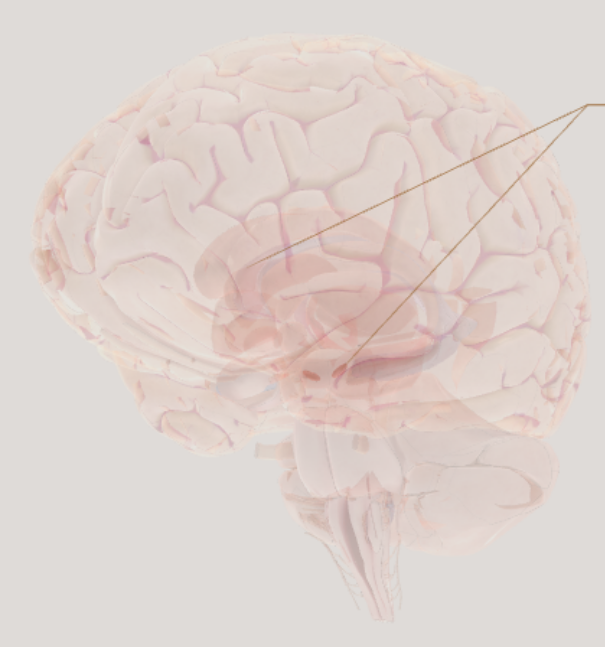
\includegraphics[width=\linewidth]{sub-n.png}
		\caption{Susbtantia nigra}
		\label{fig:subs-nig}
	\end{minipage}
	\hspace{0.5cm}
	\begin{minipage}[b]{0.5\linewidth}
		\centering
		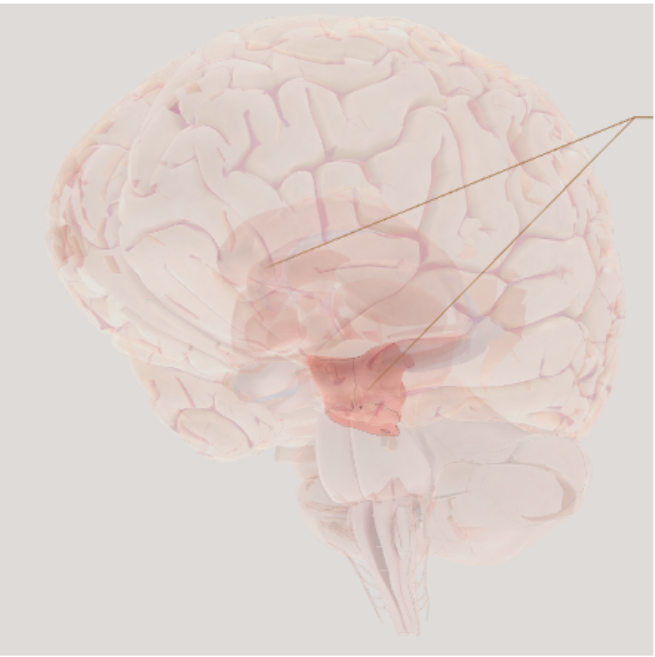
\includegraphics[width=\linewidth]{mesenc.png}
		\caption{Mesencéfalo}
		\label{fig:mesenc}
	\end{minipage}
\end{figure}



Estas neuronas dopaminérgicas tienen principalmente la función de regular la actividad motora por medio de la síntesis y la secreción de dopamina, por lo que cuando mueren se manifiestan los típicos signos de la enfermedad que nos resultan familiares: temblores, lentitud en el movimiento (bradiquinesia), inestabilidad, caídas frecuentes... A nivel macroscópico esto se manifiesta en la pérdida de pigmentación característica de la SNpc.

\begin{figure}[H] %con el [H] le obligamos a situar aquí la figura
	\centering
	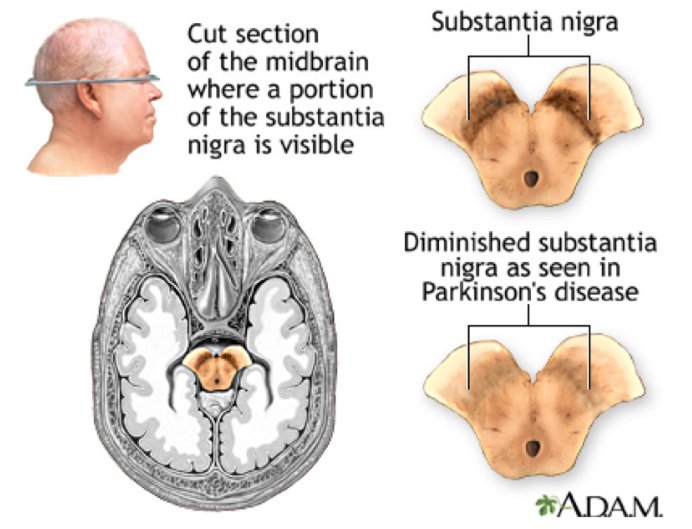
\includegraphics[scale=0.4]{pigme.png}  %el parámetro scale permite agrandar o achicar la imagen. En el nombre de archivo puede especificar directorios
	\caption{Pérdida de la pigmentación} 
	\label{fig:pigmentacion}
\end{figure}

Cabe destacar que en las neuronas supervivientes, a nivel microscópico se observan los característicos cuerpos de Lewy, que son unas ``bolsitas'' de proteínas que se acumulan en el citoplasma o cuerpo de la célula.

\begin{figure}[H] %con el [H] le obligamos a situar aquí la figura
	\centering
	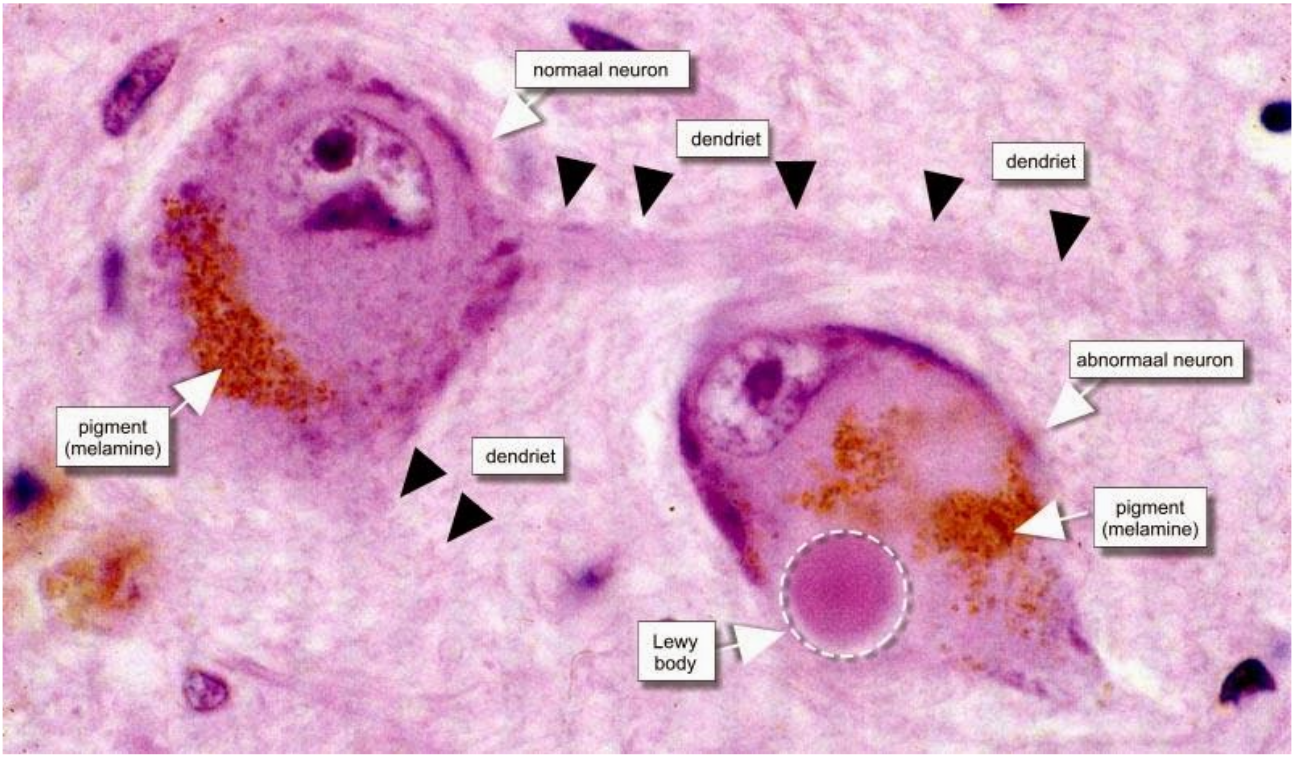
\includegraphics[scale=0.3]{cito.png}  %el parámetro scale permite agrandar o achicar la imagen. En el nombre de archivo puede especificar directorios
	\caption{Cuerpos de Lewy en el citoplasma} 
	\label{fig:lewy}
\end{figure}

\subsection{Corteza cerebral y ganglio basal}

La primera capa que nos encontramos al explorar el cerebro humano es la materia dura, esto es, una membrana que envuelve al cerebro, siendo la última capa de las meninges, cubriendo y por tanto protegiendo el cerebro y la médula espinal. Bajo esta membrana encontramos el cortex, formado por millones de neuronas de un color gris claro (la materia gris) organizadas en seis capas de entre dos y cuatro milímetros de grosor. La corteza cerebral juega un papel trascendental en la conciencia, el pensamiento, el lenguaje, la memoria, la percepción y la atención. La materia gris es una componente muy importante de nuestro sistema nervioso central. Por otra parte, la materia blanca está formada por axones que interconectan las neuronas en diferentes regiones de la corteza y del sistema nervioso central. \\

La corteza cerebral se divide en cuatro lóbulos: \\

\begin{itemize}
	\item Lóbulo temporal: Clave en la percepción auditiva, comprensión del lenguaje, memoria y aprendizaje. Contiene el hipocampo.
	\item Lóbulo frontal: Corteza motora primaria, contiene también la mayoría de las neuronas dopaminérgicas en el cortex.
	\item Lóbulo pariental: esencial para la visión espacial, la navegación y el sentido del tacto.
	\item Lóbulo occipital: Cortex visual primario, responsable de la creación de los sueños.
\end{itemize}

\begin{figure}[H] %con el [H] le obligamos a situar aquí la figura
	\centering
	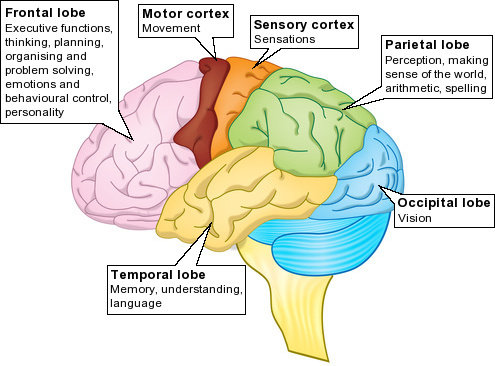
\includegraphics[scale=0.6]{bl.jpg}  %el parámetro scale permite agrandar o achicar la imagen. En el nombre de archivo puede especificar directorios
	\caption{Lóbulos de la corteza cerebral} 
	\label{fig:bl}
\end{figure}

Las neuronas dopaminérgicas de la SNpc proyectan sus axones hacia el ganglio basal, formando así el sistema dopaminérgico nigroestriatal. El ganglio basal, que se encuentra en estrecha relación con la SNpc, está descrito como la estructura cerebral más afectada por PD. Cumple un papel esencial tanto en la ejecución de movimientos voluntarios como en actividades cognitivas, por lo que su deterior asociado a PD afectará a estas funciones. \\

El ganglio basal puede verse afectado según el subtipo de la enfermedad. Hay algunos enfermos que sufren cambios microestructurales en la substantia nigra mientras que en otros apenas se aprecia. En general, el ganglio basal acaba por atrofiarse. 

\begin{figure}[H] %con el [H] le obligamos a situar aquí la figura
	\centering
	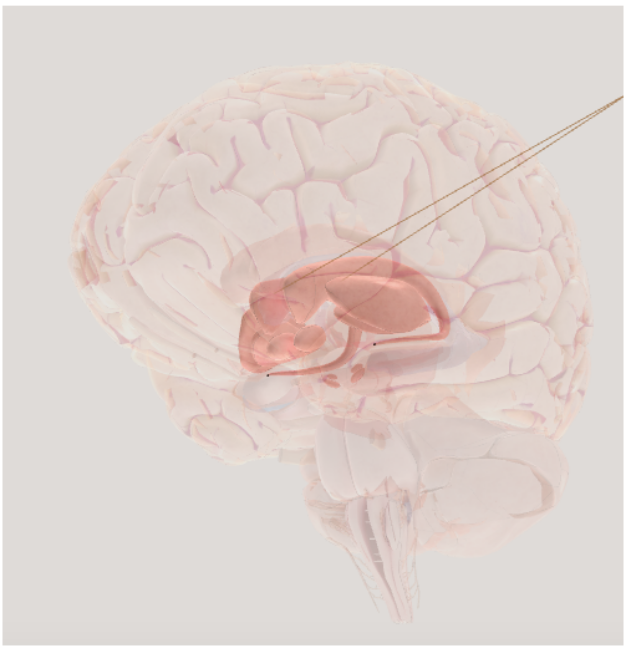
\includegraphics[scale=0.6]{gb.png}  %el parámetro scale permite agrandar o achicar la imagen. En el nombre de archivo puede especificar directorios
	\caption{Ganglio basal} 
	\label{fig:gb}
\end{figure}

Según \cite{wp}, los pacientes de PD muestran anisotropía fraccional reducida en la substantia nigra y aumento de la difusividad media y radial en la substantia nigra y el globo pálido (parte del ganglio basal), cuyos efectos pueden verse en técnicas de imagen tales como tractografías.

\subsection{Estadios del Parkinson}

La enfermedad de Parkinson afecta al ser humano de muy distintas maneras. Los enfermos no tienen por qué sufrir los mismos síntomas y, si lo hicieran, tampoco tienen por qué experimentarlos en el mismo orden ni con la misma intensidad. Sin embargo, existen algunos patrones típicos en el progreso de la enfermedad divididos en estadios \cite{wp}:

\begin{itemize}
	\item Estadio uno: Durante este estado inicial, la persona tiene síntomas menores que no interfieren en su vida diaria. Pueden darse temblores y movimientos involuntarios en un lado del cuerpo. De igual manera, se producen cambios posturales, en la forma de andar y en la expresión facial.
	\item Estadio dos: Los síntomas empeoran. Aparecen temblores, rigidez y movimientos involuntarios en ambos lados del cuerpo.
	\item Estadio tres: Considerado el estadio medio, se caracteriza por la ralentización de los movimientos y la pérdida del equilibrio. Las caídas empiezan a ser comunes.
	\item Estadio cuatro: En este punto, los síntomas son severos. Es posible permanecer de pie sin ayuda, pero en general se necesita un andador para desplazarse. La persona es incapaz de vivir sola y requiere asistencia.
	\item Estadio cinco: Este es el estadio más avanzado. Es imposible andar o ponerse de pie por la debilidad en las piernas. La persona requiere silla de ruedas y asistencia total para todas las actividades.
\end{itemize}

\subsection{Consecuencias en el cerebro}

Como hemos comentado, PD afecta a la substantia nigra. También reduce diferentes regiones de la materia gris en el lóbulo temporal. En la figura 2.7 podemos ver una resonancia magnética de un sujeto sano mientras que en la figura 2.8 vemos a un enfermo. Se puede observar la reducción de la materia gris en cada plano  e incluso su desaparición en algunas zonas.

\begin{figure}[H] %con el [H] le obligamos a situar aquí la figura
	\centering
	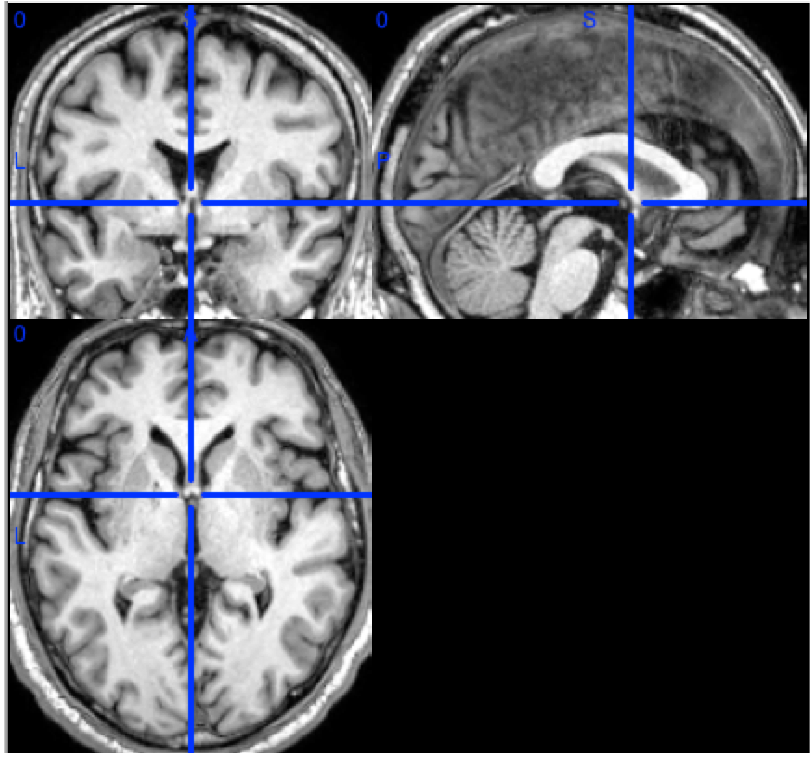
\includegraphics[scale=0.35]{healthy.png}  %el parámetro scale permite agrandar o achicar la imagen. En el nombre de archivo puede especificar directorios
	\caption{MRI de un sujeto sano} 
	\label{fig:healthy}
\end{figure}

\begin{figure}[H] %con el [H] le obligamos a situar aquí la figura
	\centering
	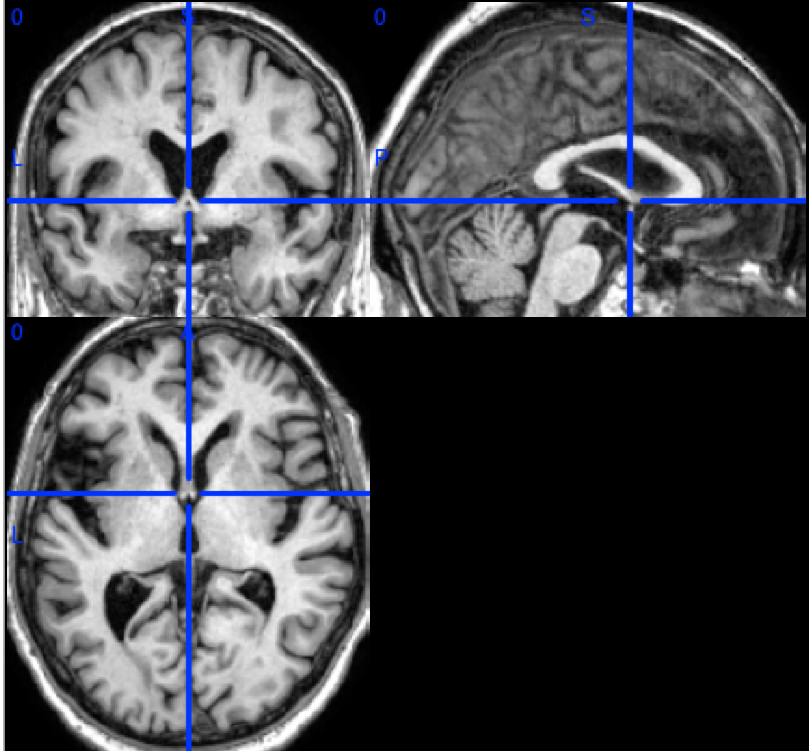
\includegraphics[scale=0.34]{unhealthy.png}  %el parámetro scale permite agrandar o achicar la imagen. En el nombre de archivo puede especificar directorios
	\caption{MRI de un sujeto enfermo de PD. Véase la pérdida de materia gris} 
	\label{fig:unhealthy}
\end{figure}

\section{Conceptos y herramientas matemáticas}

En la presente sección discutimos los diferentes conceptos y herramientas utilizadas en este proyecto. Más allá de utilizar la multitud de técnicas que existen dentro de la ciencia de datos aplicada a la biomedicina, mi intención es profundizar desde un punto de visto matemático sus fundamentos y las garantías de su uso. Primero, introduzco la imagen de resonancia magnética (MRI) y la normalización aplicada a las imágenes para los distintos experimentos. A continuación, trataré el concepto de característica en ciencia de datos y me detendré en las herramientas utilizadas para la extracción (transformada discreta Wavelets 2D) y selección (PCA) de las mismas. Por último, abordamos el tema de la clasificación, explicando el algoritmo SVM y las optimizaciones propuestas para la mejora del rendimiento,  interpretabilidad y validez de la investigación.

\subsection{Resonancia magnética nuclear}

Antes de trabajar con imágenes MRI, es necesario tener conocimiento sobre cómo se obtienen, así que introducimos los conceptos más importantes de la resonancia magnética nuclear (NMR \cite{nmr}). Se trata de un método de imagen no invasivo que tiene como objetivo obtener información sobre la estructura y composición de un material. Es muy utilizado en medicina para recabar información sobre tejidos y observar alteraciones o degradaciones de los mismos. \\

NMR es un fenómeno físico basado en las propiedades cuántico-mecánicas del núcleo atómico. Primero, el \textit{spin} (momento angular intrínseco \cite{spin}) de una partícula es un vector asociado al momento magnético de la misma. Tiene una dirección (el eje del \textit{spin}) y un sentido. Cuando dos o más partículas tienen \textit{spin} opuestos están pareadas, la suma de sus momentos es cero y, por tanto, no se produce manifestación alguna del \textit{spin}. Este es el estado natural de los momentos magnéticos en el cuerpo ya que el núcleo de los átomos y sus respectivos electrones están pareados. Sin embargo, podemos encontrar en el cuerpo isótopos con \textit{spin} distinto de cero, siendo los más comunes los de hidrógeno ya que la mayoría de los tejidos contienen agua. La manipulación del \textit{spin} es lo que permite a la máquina de resonancia magnética encontrar las diferencias entre las orientaciones y construir una imagen. Usando campos magnéticos, los núcleos de hidrógeno se alinean magnéticamente, produciéndose este cambio en las alineaciones en un tiempo T1. En presencia de un campo magnético externo, existen dos tipos de orientaciones para el \textit{spin} nuclear:

\begin{itemize}
	\item Paralela, en la que el sentido del momento magnético es el mismo para la partícula y para el campo magnético externo.
	\item Anti-paralelo, cuando ambos dos tienen sentido contrario.
\end{itemize}

Como se muestra en la Figura 3.1, la suma de los momentos magnéticos de un grupo de núcleos de hidrógeno puede ser representado como un vector M paralelo al campo magnético externo $B_0$, donde las componentes normales de los diferentes \textit{spin} se cancelan mutuamente. La mayoría de los \textit{spin} adoptan la orientación paralela, por lo que la suma de los \textit{spins} de M es paralela a $B_0$. \\

M puede ser manipulado usando señales de radio frecuencia. Cuando se aplican, los núcleos absorben la energía y una porción de ella se emite más tarde. Esa es la señal que se detecta. Dependiendo de la intensidad de los campos magnéticos, se pueden obtener imágenes con distintas resoluciones.

 \begin{figure}[H] %con el [H] le obligamos a situar aquí la figura
 	\centering
 	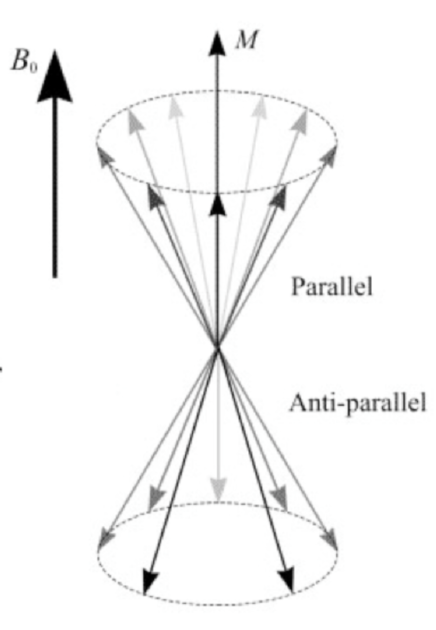
\includegraphics[scale=0.34]{nmr.png}  %el parámetro scale permite agrandar o achicar la imagen. En el nombre de archivo puede especificar directorios
 	\caption{Funcionamiento de los campos magnéticos, spin y NMR} 
 	\label{fig:nmr}
 \end{figure}

\subsection{Datos de entrada: PPMI}

A pesar de no ser una herramienta matemática, no puedo pasar sin mencionar, y al mismo tiempo agradecer, a \textit{Parkinson's Progression Makers Initiative} (PPMI). PPMI es un estudio clínico de gran importancia que evalúa las zonas cerebrales de interés usando técnicas avanzadas de imagen, muestreos biológicos y comportamientos y ensayos clínicos para identificar biomarcadores de la enfermedad del Parkinson. PPMI se lleva a cabo en Estados Unidos, Europa, Israel y Australia y, en nuestro caso, evaluó el proyecto para cedernos el acceso a su base de datos (adni.loni.usc.edu), adscrita a la Universidad Sur de California. \\

Descargamos más de 300 imágenes 3D cerebrales en formato DICOM. DICOM es el acrónimo de \textit{Digital Imaging and Communications in Medicine}. Es, al mismo tiempo, un protocolo de comunicación y un formato de archivo, lo que significa que almacena información médica, como imágenes MRI, junto con la información personal del paciente. El formato garantiza que todos esos datos se mantienen juntos, haciendo posible la transferencia de los mismos entre los profesionales. Tras eliminar archivos corruptos y duplicados, obtuvimos un dataset de 242 imágenes (78 pacientes en el grupo de control y 164 enfermos de Parkinson). 


\subsection{Normalización}

Antes de manipular o extraer información, es fundamental normalizar el conjunto de datos completo para poder comparar las imágenes. Cada imagen MRI debería representar el mismo espacio, i.e., cada región de la imagen debe describir la misma región del cerebro. Los ventrículos cerebrales deben estar situados en las mismas coordenadas para cada imagen de cada paciente. \\

Dado que los cerebros pueden variar mucho entre pacientes, este objetivo es difícil de conseguir ya que las herencia genética y la vida de cada paciente haga que cada uno tenga sus peculiaridades. Por tanto, debemos tener en cuenta dos ideas a cumplir:

\begin{itemize}
	\item Normalizar la escala de grises de las imágenes para que todas estén en la misma escala.
	\item Redimensionar las imágenes para que todas tengan las mismas medidas.
\end{itemize}

Para completar estas dos tareas, nos remitimos a una plantilla estándar. Para la normalización, utilizamos Statistical Parametric Mapping (SPM \cite{spm}), que es un algoritmo que analiza cada \textit{voxel} usando un test estadístico estándar. Lo utilizamos dada su gran efectividad y su librería de Matlab (a pesar de que el resto del proyecto se realiza en Python). Los valores de los \textit{voxel} son distribuidos de acuerdo a una función de densidad, que suele provenir de las distribuciones T de Student o F. En la Figura 3.2 podemos ver un ejemplo de una imagen antes y después de la normalización. Otra de las acciones importantes llevadas a cabo sobre los datos es una segmentación que divide genera las imágenes con su contenido completo, la materia gris (C1) y la materia blanca (C2).

 \begin{figure}[H] %con el [H] le obligamos a situar aquí la figura
	\centering
	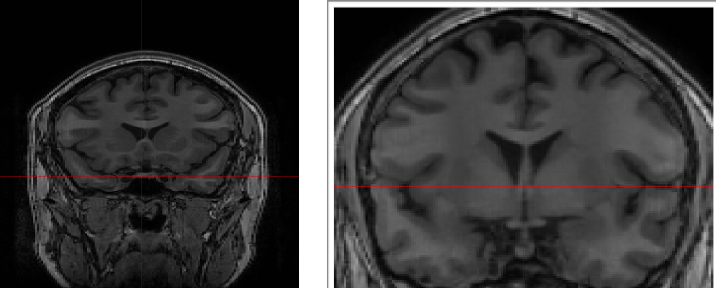
\includegraphics[scale=0.6]{norm.png}  %el parámetro scale permite agrandar o achicar la imagen. En el nombre de archivo puede especificar directorios
	\caption{A la izquierda, imagen MRI sin normalizar. A la derecha, resultado de la normalización} 
	\label{fig:norm}
\end{figure}

\subsection{Características}

Una de las partes más importantes de un proyecto de inteligencia artificial es la extracción de características. Una característica puede ser entendida como una componente de un vector, que representaría los datos. Cada elemento o individuo del dataset sería representado por un vector n-dimensional (una matriz) en la que cada componente sería una característica. Esta forma de representación es muy intuitiva y flexible ya que permite la introducción y aplicación de conceptos y herramientas matemáticas. \\

El dataset completo sería definido, una vez que cada elemento está representado por sus características, como un conjunto de vectores de $m$ componentes

$$F_i = [f_1,f_2,\dots,f_m]$$

En la expresión, $F_i$ sería un único vector (un paciente) y $f_i$ sus características. Por tanto, si tenemos un grupo de pacientes:

$$F =  \begin{pmatrix}
F_{1} \\
F_{2} \\
\vdots \\
F_{n}
\end{pmatrix} = \begin{pmatrix}
f_{11}& f_{12}& \dots& f_{1m} \\
f_{21}&f_{22}&\dots&f_{2m} \\
\vdots& \vdots& \ddots& \vdots \\
f_{n1}&f_{n2}&\dots&f_{nm}
\end{pmatrix}$$

\subsubsection{Extracción de características}

Cuando se trabaja con MRI, se tiene un número de imágenes de $157\times189\times136$ en los planos X,Y y Z respectivamente, por lo que tenemos 157*189*136 = 4.035.528 \textit{voxels} con 255 valores posibles. De esta manera encontraríamos más de mil millones de características. Necesitamos, por tanto, reducir el espacio de posibilidades, es decir, disminuir la cantidad de recursos necesaria para describir nuestro conjunto de datos. \\

En general, una buena estrategia para extraer características de una imagen es convertirla a un dominio diferente. Con ese objetivo, introducimos ahora dos opciones distintas: la transformada de Fourier y la transformada Wavelets (que finalmente utilizaremos). Todo el material aquí recogido proviene de multitud de textos. Son los siguientes: \cite{math-image}, \cite{canada}, \cite{daube}, \cite{castro}, \cite{misiti}.

\begin{itemize}
	\item \textbf{La Transformada de Fourier en $L^1(\mathbb{R}^d)$}
	
	Dado que la transformada de Fourier es, de forma natural, una función que toma valores en los complejos, asumimos que
	$$u: \mathbb{R}^d \mapsto \mathbb{C}$$
	
	\textbf{Definición 1.} Sea $u \in L^1(\mathbb{R}^d)$ y $\xi \in \mathbb{R}^d$. Se define la transformada de Fourier de $u$ en $\xi$ como 
	
	$$(F u)(\zeta) = \hat{u}(\xi) = \frac{1}{(2\pi)^{d/2}} \int_{\mathbb{R}^d} u(x) e^{-ix\xi}dx$$


Además, podemos introducir uno de los teoremas más importantes de la transformada de Fourier: el teorema de Convolución: 

\textbf{Teorema de Convolución.} Para $u, v \in L^1(\mathbb{R}^d)$,

$$ F(u*v) = (2\pi)^{d/2}F(u)F(v)$$

\textbf{Demostración.}


Aplicando el teorema de Fubini, obtenemos

$$F(u*v)(\xi) = \frac{1}{(2\pi)^{d/2}} \int_{\mathbb{R}^d} \int_{\mathbb{R}^d} u(y) v(x-y) dy\text{ } e^{-ix\xi} dx = $$
$$ == \frac{1}{(2\pi)^{d/2}} \int_{\mathbb{R}^d} \int_{\mathbb{R}^d} u(y)e^{-iy\xi}v(x-y)e^{-i(x-y)\xi}dxdy$$
$$ = \int_{\mathbb{R}^d} u(y) e^{-iy\xi} dy F(v)(\xi)$$
$$ = (2\pi)^{d/2}F(u)F(v)(\xi)$$

\hfill$\blacksquare$

A pesar de este resultado, nos será de gran utilidad extender el concepto de transformada de Fourier al espacio de Hilbert $L^2(\mathbb{R}^d)$.

\item \textbf{La Transformada de Fourier en $L^2(\mathbb{R}^d)$}

La extensión de la transformada de Fourier al espacio $L^2(\mathbb{R}^d)$ requiere un poco más de esfuerzo. En primer lugar, definimos un ``pequeño'' espacio de funciones donde la transformada exhibe ciertas propiedades interesantes: el espacio de Schwartz:

\textbf{Definición 2.} El espacio de Schwartz se define como 

$$S(\mathbb{R}^d) = \{u \in C^\infty(\mathbb{R}) | \forall \alpha,\beta \in \mathbb{N}^d: C_{\alpha,\beta}(u) = sup_{x \in \mathbb{R}^d} |x^\alpha \frac{\partial^\beta}{\partial x^\beta}u(x)| < \infty \}$$

Una función $u \in S(\mathbb{R}^d)$ se le llama una función de Schwartz.\\

\textit{Grosso modo}, el espacio de Schwartz contiene funciones suaves que tienden a cero más rápido que los polinomios a infinito. Puede verificarse de forma elemental que el espacio de Schwartz es un espacio vectorial. Con el objetivo de hacerlo accesible por métodos analíticos, lo dotamos de una topología. Describimos dicha topología definiendo una noción de \\convergencia para sucesiones de funciones.

\textbf{Definición 3.} Una sucesión de funciones de Schwartz ${u_n}$ converge a $u$ si y sólo si, para todo multi-índice $\alpha, \beta$, se tiene que 

$$C_{\alpha,\beta}(u_n - u) \mapsto 0 \text{    cuando } n \mapsto \infty$$

La convergencia en el espacio de Schwartz es muy restrictiva: una sucesión de funciones converge si ella y todas sus derivadas multiplicadas por monomios arbitrarios convergen uniformemente. 

Los siguientes lemas serán necesarios en el desarrollo del tema:

\textbf{Lema 1.} El espacio de Schwartz es no vacío y cerrado con respecto a la derivación de cualquier orden y la multiplicación usual.

\textbf{Demostración.} Para $u \in S(\mathbb{R}^d)$, para todo multi-índice $\gamma$, tenemos 

$$C_{\alpha,\beta}(\frac{\partial^\gamma}{\partial x^\gamma}u) = C_{\alpha,\beta+\gamma}(u) < \infty$$

y por tanto $\frac{\partial^\gamma}{\partial x^\gamma}u \in S(\mathbb{R}^d)$. \\

El hecho de que dadas $u, v \in S(\mathbb{R}^d)$, $uv \in S(\mathbb{R}^d)$ puede probarse vía la regla de Leibniz para multi-índices.

\hfill$\blacksquare$

El espacio de Schwartz está muy relacionado con la transformada de Fourier. El siguiente lema presenta reglas de cálculo para transformadas de Fourier sobre funciones de Schwartz.

\textbf{Lema 2.} Sea $u \in S(\mathbb{R}^d), \alpha \in \mathbb{N}^d$ un multi-índice. Se define $p^\alpha(x) = x^\alpha$. Entonces

$$F(\frac{\partial^\alpha u}{\partial x^\alpha}) = i^{|\alpha|}p^\alpha F(u)$$

$$F(p^\alpha u) = i^{|\alpha|} \frac{\partial^\alpha }{\partial x^\alpha} F(u)$$

\textbf{Demostración.}
	Comenzamos con los siguientes cálculos auxiliares:
	
	$$\frac{\partial^\alpha }{\partial x^\alpha} (e^{-ix\xi}) = (-i)^{|\alpha|} \xi^\alpha e^{-ix\xi}$$
	
	$$x^\alpha e{ix\xi} = i^{|\alpha|}\frac{\partial^\alpha}{\partial \xi^\alpha}(e^{-ix\xi})$$
	
	Aplicando integración por partes, obtenemos
	
	$$F(\frac{\partial^\alpha}{\partial x^\alpha}u)(\xi) = \frac{1}{(2\pi)^{d/2}}\int_{\mathbb{R}^d} \frac{\partial^\alpha}{\partial x^\alpha} u(x) e^{-ix\xi}dx$$
	$$= \frac{1}{(2\pi)^{d/2}} i^{|\alpha|}\xi^\alpha \int_{\mathbb{R}^d} u(x) e^{-ix\xi}dx$$
	$$=i^{|\alpha|} p^\alpha Fu(\xi)$$
	
Intercambiando el orden de la integración y la derivación, llegamos a

$$F(p^\alpha u)(\xi) = \frac{1}{(2\pi)^{d/2}}\int_{\mathbb{R}^d} u(x)x^\alpha e^{-ix\xi}dx$$
$$=\frac{1}{(2\pi)^{d/2}}\int_{\mathbb{R}^d} u(x)\frac{\partial^\alpha}{\partial \xi^\alpha}e^{-ix\xi}dx$$
$$=i^{|\alpha|}(\frac{\partial^\alpha}{\partial \xi^\alpha}Fu)(\xi)$$

Los argumentos anteriores son válidos dado que los integrandos son infinitamente derivables respecto a $\xi$ e integrables respecto a $x$.

\hfill$\blacksquare$

Observamos que la transformada de Fourier lleva diferenciación a multiplicación y viceversa. Esto nos lleva a que el espacio de Schwartz va a sí mismo vía la transformada de Fourier. Veámoslo:\\

\textbf{Lema 3.} Para la función $G(x) = e^{-\frac{|x|^2}{2}}$, se tiene que 

$$\hat{G}(\xi) = G(\xi)$$

es decir, la función Gaussiana es una función propia de la transformada de Fourier correspondiente al valor propio uno.

\textbf{Demostración}

La función Gaussiana se puede escribir como un producto tensorial de Gaussianas unidimensionales $g:\mathbb{R} \mapsto \mathbb{R}, g(t) = exp(-t^2/2)$ de forma que $G(x) = \prod_{k=1}^{d} g(x_k)$. Por el teorema de Fubini,

$$\hat{G}(\xi) = \frac{1}{(2\pi)^{d/2}} \int_{\mathbb{R}^d} \prod_{k=1}^{d} g(x_k) e^{-i x_k \xi_k} dx = \prod_{k=1}^{d} \hat{g}(\xi_k)$$

Para calcular la transformada de Fourier de $g$, tengamos en cuenta que $g$ satisface la ecuación diferencial $g'(t) = -t g(t)$. Aplicando la transformada de Fourier en esa ecuación, por el Lema 2 obtenemos $-\omega \hat{g}(\omega) = \hat{g}'(\omega)$. De hecho, $\hat{g}(0) = \int_{\mathbb{R}}g(t) dt = 1 = g(0)$. Por tanto, las funciones $g,\hat{g}$ satisfacen la misma ecuación diferencial con el mismo valor inicial. Por el teorema de unicidad de soluciones en problemas de valores iniciales de Picard-Lindelöf, $g = \hat{g}$.

\hfill$\blacksquare$

\textbf{Teorema 2.} La transformada de Fourier es una aplicación continua y biyectiva del espacio de Schwartz en sí mismo. Para $u \in S(\mathbb{R}^d)$, tenemos la fórmula de inversión

	$$(F^{-1}Fu)(x) = \overline{\hat{u}}(x)= \frac{1}{(2\pi)^{d/2}} \int_{\mathbb{R}^d} \hat{u}(\xi) e^{ix\xi} d\xi = u(x)$$

\textbf{Demostración.} Por el lema 2, tenemos que para todo $\xi \in \mathbb{R}^d$

$$|\xi^\alpha \frac{\partial^\beta}{\partial \xi^\beta}\hat{u}(\xi)| = |F(\frac{\partial^\alpha}{\partial x^\alpha}p^\beta u)(\xi)| \leq \frac{1}{(2\pi)^{d/2}} \left\Vert \frac{\partial^\alpha}{\partial x^\alpha}p^\beta u \right \Vert_1  (*)$$

Por tanto, para $u \in S(\mathbb{R}^d)$, tenemos que $\hat{u} \in S(\mathbb{R}^d)$. Dado que la transformada de Fourier es lineal, es suficiente demostrar la continuidad en el cero. En efecto, consideramos a sucesión nula ${u_n}$ en el espacio de Schwartz, es decir, cuando $n \mapsto \infty, C_{\alpha,\beta}(u_n) \mapsto 0$. Esto es, ${u_n}$, al igual que ${\partial^\alpha p^\beta u_n}, \forall \alpha, \beta$, converge uniformemente a cero. Esto implica que la parte derecha de $(*)$ tiende a cero. En particular, obtenemos que $C_{\alpha,\beta}(\hat(u_n)) \mapsto 0$, lo que implica que ${\hat{u_n}}$ es una sucesión nula, probando la continuidad. \\

Para probar la fórmula de inversión, consideramos dos funciones arbitrarias $u, \phi \in S(\mathbb{R}^d)$

$$(\hat{\hat{u}}*\phi)(x) = \int_{\mathbb{R}^d} \hat{\hat{u}}(y) \phi(x-y) dy = \int_{\mathbb{R}^d}\hat{u}(y) e^{ixy} \hat{\phi}(-y) dy$$
$$ = \int_{\mathbb{R}^d} u(y) \hat{\hat{\phi}}(-x-y)dy = (u*\hat{\hat{\phi}})(-x)$$

Ahora elegimos $\phi$ para que sea una función Gaussiana reescalada:

$$\phi_{\epsilon}(x) = \epsilon^{-d}(D_{\epsilon^{-1}id}G)(x) = \epsilon^{-d}e^{-\frac{|x|^2}{2\epsilon^2}}$$

De estos cálculos inferimos que $\hat{\phi}_\epsilon = D_{\epsilon\text{ } id}\hat{G}$ y por tanto $\hat{\hat{\phi}}_\epsilon = \epsilon^{-d} D_{\epsilon^{-1}\text{ } id}\hat{\hat{G}}$. Por el lema 3, $\hat{G} = G$ y $\hat{\hat{\phi_{\epsilon}}} = \phi_{\epsilon}$. Dado que $u$ es en particular acotada y continua, y G es positiva con integral normalizada a uno, podemos aplicar las propiedades de la convolución y obtener que cuando $\epsilon \mapsto 0$,

$$\hat{\hat{u}}*\phi_{\epsilon}(x) \mapsto \hat{\hat{u}}(x)  \text{ y } u*\phi_{\epsilon}(-x) \mapsto u(-x) \Rightarrow \hat{\hat{u}}(x)=u(-x) $$

Por propiedades de conjugación de la transformada de Fourier, tenemos que $\overline{u} = D_{-id} \hat{u}$ y sustituyendo $\hat{u}$ por $u$, obtenemos:

$$\overline{\hat{u}} = D_{-id} \hat{\hat{u}} = u$$


\hfill$\blacksquare$

\textbf{Teorema 3.} Hay un único operador $F:L^2(\mathbb{R}^d) \mapsto L^2(\mathbb{R}^d)$ que extiende la transformada de Fourier $F$ a $S(\mathbb{R}^d)$ y satisface la ecuación $\left\Vert u \right \Vert_2 = \left\Vert Fu \right \Vert_2 \forall u \in L^2(\mathbb{R}^d)$. Además, $F$ es biyectivo y su inversa $F^{-1}$ es una extensión continua de $F^{-1}$ en $S(\mathbb{R}^d)$

\textbf{Demostración.} Para $u,v \in S(\mathbb{R}^d)$, sabemos que 

$$(\hat{u},\hat{v})_2 = (u,v)_2$$

y en particular $\left \Vert u \right \Vert_2 = \left \Vert Fu \right \Vert_2$. Por tanto, la transformada de Fourier es una isometría definida en un subconjunto  denso de $L^2(\mathbb{R}^d)$. Existe una única extensión continua en todo el espacio. Debido a la simetría entre $F$ y $F^{-1}$, un argumento análogo demuestra el recíproco.

\hfill$\blacksquare$

La propiedad de isometría $\left \Vert u \right \Vert_2 = \left \Vert Fu \right \Vert_2$ también implica que

$$(u,v)_2 = (Fu,Fv)_2$$
que se conoce como la fórmula de Plancherel.

\item \textbf{Transformada Wavelet}

En la sección anterior tratamos los fundamentos teóricos que sostienen la transformada de Fourier como herramienta para estudiar la representación de la frecuencia de una señal o imagen. Sin embargo, la información relacionada con la localización no es codificada de una forma plausible. En particular, una alteración local de una señal o una imagen da lugar a una modificación global de toda la transformada de Fourier. En otras palabras, la transformada de Fourier es una transformación global en el sentido de que $\hat{u(\xi)}$ depende de todos los valores de $u$. En ciertas circunstancias, las transformaciones locales son deseables. Antes de introducir nuestra herramienta fundamental en la extracción de características, la transformada Wavelet, presento una nueva alternativa para estudiar información ``local'' en la frecuencia: la transformada de Fourier de tiempo reducido o transformada ``ventana'' de Fourier (\cite{stft}):

\textbf{Definición 4.} Sean $u,g \in L^2(\mathbb{R}^d)$. La transformada de Fourier de tiempo reducido de $u$ con una función ventana $g$ se define como

$$(G_g u)(\xi,t) = \frac{1}{(2\pi)^{d/2}}\int_{\mathbb{R}^d} u(x) \overline{g(x-t)} e^{-ix\xi}dx$$

Esta transformada depende de un parámetro de frecuencia $\xi$ y de un parámetro espacial $t$ y existen muchas formas de representarla:

$$(G_g u)(\xi,t) = F(uT_{-t} \overline{g})(\xi)$$
$$ = \frac{1}{(2\pi)^{d/2}} (u, M_\xi T_{-t}g)_2$$
$$ =  \frac{1}{(2\pi)^{d/2}} (M_{-\xi}u*D_{-id}\overline{g})(t)$$

La primera alternativa explica el nombre de ``ventana'': a través de la multiplicación por la función $g$, $u$ es localizada previa la transformada de Fourier. Nótese que la transformada ``ventana'' de Fourier es una función de $2d$ variables: $(G_g u): \mathbb{R}^{2d} \mapsto \mathbb{C}$. \\

\textbf{Lema 4.} Sean $u,v,g \in L^2(\mathbb{R}^{2d})$. Entonces  $(G_g u) \in L^2(\mathbb{R}^{2d})$ y 

$$(G_g u, G_g v)_{L^2(\mathbb{R}^{2d})} = \Vert g \Vert_2^2(u,v)_2$$

\textbf{Demostración.} Para probar la igualdad entre productos escalares, usamos la isometría de la transformada de Fourier y la fórmula de Plancherel. Con $F_t$ denotamos la transformada de Fourier respecto de $t$, utilizamos una de las alternativas de representación de la transformada ventana de Fourier y el teorema de convolución para obtener

$$F_t(G_g u(\xi,·))(\omega) = F_t((2\pi)^{d/2}(M_{-\xi}u*D_{-id}\overline{g}))(\omega)$$
$$= F(M_{-\xi}u)(\omega)(F D_{-id}\overline{g})(\omega)$$
$$= \hat{u}(\omega+\xi)\overline{\hat{g}}(\omega)$$

Obtenemos el resultado con el siguiente cálculo:

$$(G_g u,G_g v)_{L^2(\mathbb{R}^{2d})} = (F_t(G_g u), F_t(G_g v))_{L^2(\mathbb{R}^{2d})}$$
$$ = \int_{\mathbb{R}^d} \int_{\mathbb{R}^d} \hat{u}(\omega + \xi) \overline{\hat{g}}(\omega) \overline{\hat{v}}(\omega+\xi)\hat{g}(\omega) d\xi d\omega$$
$$= \int_{\mathbb{R}^d} |\hat{g}(\omega)|^2 \int_{\mathbb{R}^d} \hat{u}(\omega+\xi) \overline{\hat{v}}(\omega+\xi) d\xi d\omega$$
$$=\Vert \hat{g} \Vert_2^2(\hat{u},\hat{v})_2$$
$$=\Vert \hat{g} \Vert_2^2(u,v)_2$$

\hfill$\blacksquare$


Vemos entonces que la transformada de Fourier de tiempo reducido es una isometría, por lo que podemos calcular la fórmula de inversión:

\textbf{Corolario 1.} Para $u,g \in L^2(\mathbb{R}^d)$ con $\Vert g \Vert_2 = 1$, tenemos que la fórmula de inversión es

$$u(x) = \frac{1}{(2\pi)^{d/2}} \int_{\mathbb{R}^d} \int_{\mathbb{R}^d} G_g u(\xi,t) g(x-t) e^{ix\xi} d\xi dt \text{    para casi todo x.}$$


\textbf{Demostración.} Dado que $g$ está normalizada, $G_g$ es una isometría, por lo que sólo nos queda calcular el operador adjunto. Para $u \in L^2(\mathbb{R}^d)$ y $F \in L^2(\mathbb{R}^{2d})$, tenemos que

$$ (u, G_g^*F)_{L^2(\mathbb{R}^d)} = (G_g u,F)_{L^2(\mathbb{R}^{2d})}$$
$$ = \int_{\mathbb{R}^{2d}} G_g u(\xi,t) \overline{F(\xi,t)} d\xi dt$$
$$ = \int_{\mathbb{R}^{2d}} \frac{1}{(2\pi)^{d/2}} \int_{\mathbb{R}^{2d}} u(x) \overline{g(x-t)} e^{-ix \xi}dx \overline{F(\xi,t)} d\xi dt$$
$$ = \int_{\mathbb{R}^d} u(x) \overline{\frac{1}{(2\pi)^{d/2}} \int_{\mathbb{R}^{2d}} F(\xi,t) e^{ix\xi}g(x-t)d\xi dt} dx,$$

lo que implica

$$G_g^*F(x) = \frac{1}{(2\pi)^{d/2}} \int_{\mathbb{R}^{2d}} F(\xi,t) e^{ix\xi}g(x-t)d\xi dt$$

\hfill$\blacksquare$

La transformada ventana de Fourier no se aplica en procesamiento de imágenes generalmente. Hay varios motivos: en primer lugar, la transformación de una imagen produce una función de cuatro variables. Esto nos lleva a un gran consumo de memoria y perdemos gran parte de la capacidad de visualización. Por otra parte, la discretización de esta transformada no es para nada trivial y no hay un análogo directo para series de Fourier o transformada discreta. Para más información, véase (\cite{ftta}).

\item Transformada Wavelet continua

Nos centramos a partir de ahora en la herramienta principal en cuanto a la extracción de características se refiere. Mientras que la transformada de tiempo reducido de Fourier usa una ventana fija para localizar la función de interés, la transformada wavelet utiliza funciones variando sus anchuras (Figura 3.3). 

 \begin{figure}[H] %con el [H] le obligamos a situar aquí la figura
	\centering
	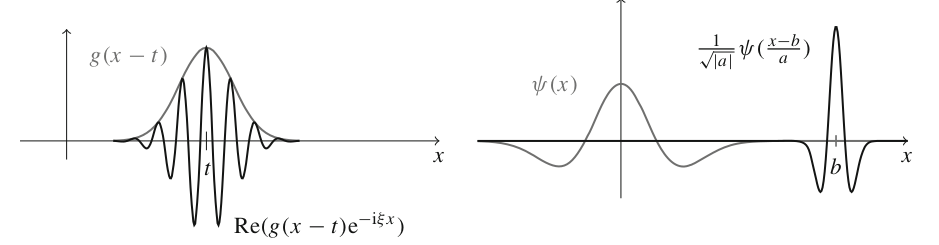
\includegraphics[scale=0.42]{widths.png}  %el parámetro scale permite agrandar o achicar la imagen. En el nombre de archivo puede especificar directorios
	\caption{Transformada ventana (izquierda) y transformada wavelet (derecha)} 
	\label{fig:widths}
\end{figure}

En el caso de que nos encontremos en dimensión mayor que uno (nuestro caso), la transformada se puede definir de varias formas. Nos ocupamos primero de la transformada unidimensional:

\textbf{Definición 5.} Sean $u, \psi \in L^2(\mathbb{R},\mathbb{R})$. Para $b \in \mathbb{R}, a>0$ la transformada wavelet de $u$ con $\psi$ se define como

$$L_\psi u(a,b) = \int_{\mathbb{R}} u(x) \frac{1}{\sqrt{a}} \psi\left(\frac{x-b}{a}\right) dx$$

La transformada wavelet depende del parámetro espacial $b$ y el parámetro de escala $a$. Como en casos anteriores, podemos representarla de múltiples formas:

$$L_\psi (a,b) = \frac{1}{\sqrt{a}} (u, T_{-b}D_{1/a}\psi)_{L^2(\mathbb{R})}$$
$$=\frac{1}{\sqrt{a}} (u*D_{-1/a}\psi)(b))$$

Como la transformada de Fourier de tiempo reducido, la transformada wavelet posee cierta isometría, sin embargo, lo hace respecto de una medida ponderada. Introduzco el siguiente espacio:

$$L^2 \left( [0,\infty[ \times \mathbb{R}, \frac{da db}{a^2}\right) = \{ F: [0,\infty[ \times \mathbb{R} \mapsto \mathbb{R}: \int_{\mathbb{R}} \int_{\mathbb{R}^+} |F(a,b)|^2 \frac{da db}{a^2} < \infty \} $$

El producto escalar en este espacio es

$$(F,G)_{L^2 \left( [0,\infty[ \times \mathbb{R}, \frac{da db}{a^2}\right)} = \int_{\mathbb{R}} \int_{\mathbb{R}^+} F(a,b) G(a,b) \frac{da db}{a^2}$$

\textbf{Teorema 4.} Sea $u, \psi \in L^2(\mathbb{R})$ con 

$$ 0 < c_\psi = 2\pi \int_{\mathbb{R}^+} \frac{|\hat{\xi}(\xi)|^2}{\xi} d\xi < \infty$$

Entonces 

$$L_\psi : L^2(\mathbb{R}) \mapsto L^2 \left( [0,\infty[ \times \mathbb{R}, \frac{da db}{a^2}\right)$$

es una función lineal y se tiene que

$$(L_\psi u, L_\psi v)_{L^2 \left( [0,\infty[ \times \mathbb{R}, \frac{da db}{a^2}\right)} = c_\psi(u,v)_{L^2\mathbb{R}}$$

\textbf{Demostración.} Usamos el producto escalar de la transformada wavelet, las propiedades de la transformada de Fourier y la fórmula de Plancherel para obtener

$$L_\psi u (a,b) = \frac{1}{\sqrt{a}}(u,T_{-b}D_{1/a}\psi)_{L^2(\mathbb{R})}$$
$$ = \frac{1}{\sqrt{a}} (\hat{u}, F(T_{-b}D_{1/a}\psi))_{L^2(\mathbb{R})}$$
$$ = \frac{1}{\sqrt{a}} (\hat{u},aM_{-b}D_a\hat{\psi})_{L^2(\mathbb{R})}$$
$$=\sqrt{a} \int_{\mathbb{R}} \hat{u}(\psi)e^{ib\psi}\overline{\hat{\psi}(a\xi)} d\xi$$
$$= \sqrt{a 2\pi} F^{-1} (\hat{u}\overline{D_a \hat{\psi}})(b)$$

Ahora, calculamos lo siguiente:

$$(L_\psi u, L_\psi v)_{ L^2 \left( [0,\infty[ \times \mathbb{R}, \frac{da db}{a^2}\right)} = \int_{\mathbb{R}}
\int_{\mathbb{R}^+} L_\psi u(a,b) L_\psi v(a,b) \frac{da db}{a^2}$$
$$= 2\pi \int_{\mathbb{R}^+} \int_{\mathbb{R}} a F^{-1}(\hat{u}\overline{D_a \hat{\psi}})(b)\overline{F^{-1}(\hat{v}\overline{D_a \hat{\psi}})(b)} db \frac{da}{a^2}$$
$$ = 2\pi  \int_{\mathbb{R}^+} \int_{\mathbb{R}}
a \hat{u}(\xi) \overline{\hat{\psi}(a\xi)}\overline{\hat{v}(\xi)\overline{\hat{\psi}(a\xi)}} d\xi \frac{da}{a^2}$$
$$ = 2\pi \int_{\mathbb{R}} \hat{u}(\xi) \overline{\hat{v}(\xi)} \int_{\mathbb{R}^+} \frac{|\hat{\psi}(a\xi)|^2}{a} da d\xi$$

Un cambio de variable y $|\hat{\psi}(-\xi)| = |\hat{\psi}(\xi)|$ lleva 

$$\int_{\mathbb{R}^+} \frac{|\hat{\psi}(a\xi)|^2}{a} da = \int_{\mathbb{R}^+} \frac{|\hat{\psi}(a|\xi|)|^2}{a} da = \int_{\mathbb{R}^+} \frac{|\hat{\psi}(\omega)|^2}{\omega} d\omega = \frac{c_\psi}{2\pi}$$

Aplicando la fórmula de Plancherel obtenemos lo que buscábamos.

\hfill$\blacksquare$

Que $c_\psi < \infty$ asegura que $L_\psi$ es una función continua y $c_\psi > 0$ garantiza la existencia de la inversa de $L_\psi$. \\

\textbf{Definición 6} La condición

$$0 < c_\psi = 2\pi \int_{\mathbb{R}^+} \frac{|\hat{\psi}(\xi)|^2}{\xi} d\xi < \infty$$

se llama la condición de admisibilidad y la función $\psi$ que la satisface se le llama \textit{wavelets}.

La condición de admisibilidad dice que, alrededor de cero, la transformada de Fourier de una wavelet tiende suficientemente rápido a cero, $\hat{\psi}(0) = 0$.

\textbf{Corolario 2} Sea $u, \psi \in L^2(\mathbb{R})$ y $c_\psi = 1$. Entonces

$$u(x) = \int_{\mathbb{R}} \int_{\mathbb{R}^+} L_\psi u(a,b) \frac{1}{\sqrt{a}} \psi\left(\frac{x-b}{a}\right) \frac{da db}{a^2}$$

\textbf{Demostración.} Calculamos el adjunto de la transformada Wavelet. Para $u \in L^2(\mathbb{R})$, y $F \in L^2 \left( [0,\infty[ \times \mathbb{R}, \frac{da db}{a^2}\right)$,

$$(L_\psi u, F)_{L^2 \left( [0,\infty[ \times \mathbb{R}, \frac{da db}{a^2}\right)} = \int_{\mathbb{R}} \int_{\mathbb{R}^+} \int_{\mathbb{R}} u(x) \frac{1}{\sqrt{a}} \psi\left(\frac{x-b}{a}\right)dx F(a,b) \frac{da db}{a^2}$$
$$ = \int_{\mathbb{R}} u(x) \int_{\mathbb{R}} \int_{\mathbb{R}^+} F(a,b) \frac{1}{\sqrt{a}} \psi\left(\frac{x-b}{a}\right) \frac{da db}{a^2}dx $$

Esto implica que

$$L_\psi^* F(x) = \int_{\mathbb{R}} \int_{\mathbb{R}^+} F(a,b) \frac{1}{\sqrt{a}} \psi\left(\frac{x-b}{a}\right) \frac{da db}{a^2}$$

como queríamos demostrar.

\hfill$\blacksquare$

Presento ahora la wavelet más sencilla:

\textbf{Haar wavelet:} 

$$\psi(x) = \begin{cases}
	1 \  \ \ si \ 0 \leq x < 0.5 \\
	-1 \ \  si \ 0.5 \leq x < 1 \\
	0 \ \ en \ otro \ caso
\end{cases}$$

Es discontinua pero de soporte compacto:

\begin{figure}[H] %con el [H] le obligamos a situar aquí la figura
	\centering
	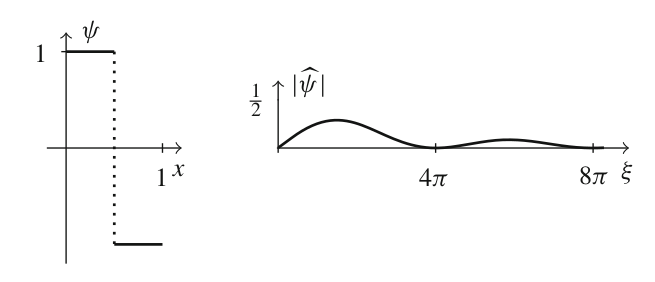
\includegraphics[scale=0.42]{haar.png}  %el parámetro scale permite agrandar o achicar la imagen. En el nombre de archivo puede especificar directorios
	\caption{Wavelet Haar} 
	\label{fig:haar}
\end{figure}

\item Transformada discreta Wavelet

La transformada continua Wavelet es una representación redundante. La pregunta que surge es si sería suficiente con conocer la transformada wavelet de una función en un subconjunto de $[0,\infty[ \times \mathbb{R}$. Este es el caso para algunos subconjuntos discretos. Veamos que bajo ciertas condiciones, las funciones

$$\{\psi_{j,k}(x) = 2^{-j/2}\psi(2^{-j}x-k) | j,k \in \mathbb{Z}\}$$

forman una base ortonormal de $L^2(\mathbb{R})$. Para demostrarlo, primero necesitamos introducir ciertos conceptos. El primo de ellos es la noción de serie wavelet y transformada discreta wavelet, a saber, lo conocido como ``análisis multiescala''. \\

\textbf{Definición 7.} Una sucesión $(V_j)_{j \in \mathbb{Z}}$ de subconjuntos cerrados de $L^2(\mathbb{R})$ es llamado un análisis multiescala si satisface las siguientes condiciones:

\begin{itemize}
	\item Invarianza por traslaciones: $$\forall j,k \in \mathbb{Z}, u_j \in V_j \Leftrightarrow T_{2^jk}u \in V_j$$
	\item Inclusión: $$\forall j \in \mathbb{Z}, V_{j+1} \subset V_{j}$$
	\item Escala: $$\forall j \in \mathbb{Z}, u \in V_{j} \Leftrightarrow D_{1/2}u \in V_{j+1}$$
	\item Intersección trivial: $$\cap_{j \in \mathbb{Z}} V_j = \{0\}$$
	\item Completitud: $$\overline{\cup_{j \in \mathbb{Z}} V_j} = L^2(\mathbb{R})$$
	\item Base ortonormal: Existe una función $\phi \in V_0$ tal que las funciones $\{T_k \phi | k \in \mathbb{Z} \}$ forman una base ortonormal de $V_0$
	La función $\phi$ es llamada un generador o una función de escala del análisis multiescala.
\end{itemize}

Hagamos algunas puntualizaciones sobre esta definición. Los espacios $V_j$ son invariantes por traslación respecto de las traslaciones diádicas $2^j$. Además, están encajadas entre sí y se hacen más pequeñas conforme crece $j$. Si notamos $P_{V_j}$ como la proyección ortogonal sobre $V_j$, entonces para todo $u$ 

$$\lim_{j \mapsto \infty} P_{V_j} u = 0, \lim_{j \mapsto -\infty} P_{V_j} u = 0$$

\textbf{Definición 8.} Sea $(V_j)_{j \in \mathbb{Z}}$ un análisis multiescala. Sean $W_j$ los espacios definidos como los complementos ortogonales de $V_j, V_{j-1}$

$$V_{j-1} = V_j \oplus W_j, V_j \perp W_j$$

El espacio $V_j$ es llamado el espacio aproximación a la escala $j$; el espacio $W_j$ es llamado el espacio wavalet a la escala $j$.

La definición de $W_j$ directamente implica

$$V_j = \oplus_{m \in \mathbb{Z}} W_m$$

y debido a la completitud de $V_j$,

$$L^2(\mathbb{R}) =   \oplus_{m \in \mathbb{Z}} W_m$$

Además, tenemos que $P_{V_{j-1}} = P_{V_j} + P_{W_j}$ y por tanto

$$ P_{W_j} = P_{V_{j-1}} - P_{V_j}$$

Podemos ahora representar cada $u \in L^2(\mathbb{R})$ a través de los espacios $V_j, W_j$ 

$$ u = \sum_{j \in \mathbb{Z}}P_{W_j}u = P_{V_m}u + \sum_{j \leq m}P_{W_j}u$$

Estas ecuaciones justifican el nombre de análisis multiescala: los espacios $V_j$ permiten una aproximación sistemática de funciones a diferentes escalas.

\textbf{Teorema 5.} Sea $(V_j)$ un análisis multiescala con generador $\phi$ tal que $\phi$ satisface 

$$\phi(x) = \sum_{j \in \mathbb{Z}} h_k \sqrt{2} \phi(2x-k)$$ 
con una sucesión $(h_k)$. Más aún, sea $\psi \in V_{-1}$ definido como

$$\psi(x) = \sqrt{2} \sum_{k \in \mathbb{Z}} (-1)^k h_{1-k}\phi(2x-k)$$

Entonces:

\begin{enumerate}
	\item El conjunto $\{\psi_{j,k}: k\in \mathbb{Z} \}$ es una base ortonormal de $W_j$.
	\item El conjunto $\{\psi_{j,k}: k\in \mathbb{Z} \}$ es una base ortonormal de $L^2(\mathbb{R})$.
	\item La función $\psi$ es una wavelet con $c_\psi = 2 \log 2$.
\end{enumerate}

\textbf{Demostración.} Primero vemos que para todo $k \in \mathbb{Z}$, tenemos que

$$(\psi, \phi_{k,0}) = 0,$$
$$(\psi, \psi_{k,0}) = \delta_{0,k}$$

La primera ecuación implica que $\psi \perp V_0$, y por tanto tenemos que $\psi \in W_0$. La segunda ecuación implica la ortonormalidad de las traslaciones de $\psi$. \\

Ahora demostramos que el sistema $\{\psi_{k,0} | k \in \mathbb{Z} \}$ es completo en $W_0$. Dado que $V_{-1} = V_0 \oplus W_0$, es equivalente demostrar que el sistema $\{\phi_{k,0} | k \in \mathbb{Z} \}$ es completo en $V_{-1}$. Esto último lo obtenemos viendo que $\phi_{-1,0}$ se puede representar como $\{\phi_{k,0}, \psi_{k,0} | k \in \mathbb{Z} \}$. Para ello, calculamos lo siguiente:

$$\sum_{k \in \mathbb{Z}} | (\phi_{-1,0}, \psi_{k,0})|^2 +  | (\phi_{-1,0}, \phi_{k,0})|^2$$
$$= \sum_{k \in \mathbb{Z}}| \sum_{l \in \mathbb{Z}} h_l (\phi_{-1,0},\phi_{-1,l+2k}) |^2 + | \sum_{l \in \mathbb{Z}}(-1)^l h_{1-l} (\phi_{-1,0},\phi_{-1,l+2k}) |^2$$
$$= \sum_{k \in \mathbb{Z}} h_{-2k}^2 + h_{1+2k}^2 = \sum_{k \in \mathbb{Z}}h_k^2$$

Se puede ver que $\sum_{k \in \mathbb{Z}} h_k^2 = 1$, y debido que $\Vert \phi_{-1,0} \Vert = 1$, se sigue que el sistema $\{\phi_{k,0}, \psi_{k,0} | k \in \mathbb{Z} \}$ es completo en $V_{-1}$.

Para el tercer punto, hago referencia a \cite{meyer}


\hfill$\blacksquare$

Por último, desarrollo la transformada wavelet discreta bidimensional, la herramienta definitiva para nuestro estudio 2D de las MRI cerebrales:

\item La Transformada Wavelet Discreta Bidimensional

Basándonos en una base wavelet ortonormal $\{\psi_{j,k} | j,k \in \mathbb{Z} \}$ de $L^2)(\mathbb{R})$, podemos construir una base ortonormal de $L^2(\mathbb{R}^2)$ a través de todos los productos tensoriales. Las funciones

$$(x_1,x_2) \mapsto \psi_{j_1,k_1}(x_1), \psi_{j_2,k_2}(x_2), \ \ \  j_i,k_i \in \mathbb{Z}$$

forman una base ortonormal de $L^2(\mathbb{R}^2)$.

En el mismo sentido, podemos constituir un análisis multiescala de $L^2(\mathbb{R}^2)$: para un análisis multiescala $(V_j)$ de $L^2(\mathbb{R}^2)$, creamos los espacios

$$V_j^2 = V_j \otimes V_j \subset L^2(\mathbb{R}^2)$$

que están definidos dado que las funciones

$$\Phi_{j,k}: (x_1,x_2) \mapsto \phi_{j,k_1}(x_1) \phi_{j,k_2}(x_2), \vspace{0.5cm} k= (k_1,k_2) \in \mathbb{Z}^2$$

forman una base ortonormal de $V_j^2$. Esta construcción también es llamada un producto tensorial para espacios de Hilbert separables (\cite{weid}). \\

En el caso bidimensional, los espacios wavelet, es decir, los complementos ortogonales de $V_j^2$ en $V_{j-1}^2$ tienen una estructura más compleja. Definimos el espacio wavelet $W_j^2$ 

$$V_{j-1}^2 = V_j^2 \oplus W_j^2$$

donde el superíndice 2 significa en un caso un producto tensorial y en el otro representa un nombre. Por otra parte, $V_{j-1} = V_j \oplus W_j$, de lo que obtenemos

$$V_{j-1}^2 = (V_j \oplus W_j) \otimes (V_j \oplus W_j)$$
$$ = (V_j \otimes V_j) \oplus (V_j \otimes W_j) \oplus (W_j \otimes V_j) \oplus (W_j \otimes W_j)$$

y llamando

$$H_j^2 = V_j \otimes W_j, \hspace{0.2cm} S_j^2 = W_j \otimes V_j, \hspace{0.2cm} D_j^2 = W_j \otimes W_j$$

podemos expresar

$$V_{j-1}^2 = V_j^2 \oplus H_j^2 \oplus S_j^2 \oplus D_j^2$$

Denotando la función de escala de $(V_j)$ como $\phi$ y la correspondiente wavelet como $\psi$, definimos tres funciones:

$$\psi^1(x_1,x_2) = \phi(x_1) \psi(x_2), \hspace{0.2cm} \psi^2(x_1,x_2) = \psi(x_1) \phi(x_2), \hspace{0.2cm} \psi^3(x_1,x_2) = \psi(x_1) \psi(x_2)$$

Para $m \in {1,2,3}, j \in \mathbb{Z}, k \in \mathbb{Z}^2$, establecemos,

$$\psi_{j,k}^2(x_1,x_2) = 2^{-j} \psi^m(2^{-j}x_1-k_1,2^{-j}x_2-k_2)$$

Se puede probar que las funciones $\{\psi_{j,k}^1 | k \in \mathbb{Z}^2 \}$ forma una base ortonormal de $H_j^2$, las funciones $\{\psi_{j,k}^2 | k \in \mathbb{Z}^2 \}$ constituyen una base de $S_j^2$ y las funciones $\{\psi_{j,k}^3 | k \in \mathbb{Z}^2 \}$, de $D_j^2$. Por tanto

$$\{\psi_{j,k}^m | m = 1,2,3, k\in \mathbb{Z}^2, j \in \mathbb{Z}\}$$

constituye de forma natural una base ortonormal de $L^2(\mathbb{R}^2)$.

Observamos que los espacios wavelet $W_j^2$ están generados por tres wavelets: $\psi^1, \psi^2$ y $\psi^3$ juntas con sus escalas y traslaciones. Los espacios $H_j^2$ contienen los detalles horizontales en la escala $j$ (en la dirección $x_1$) , los espacios $S_j^2$ los detalles verticales (dirección $x_2$) y los espacios $D_j^2$ los detalles en diagonal:

\begin{figure}[H] %con el [H] le obligamos a situar aquí la figura
	\centering
	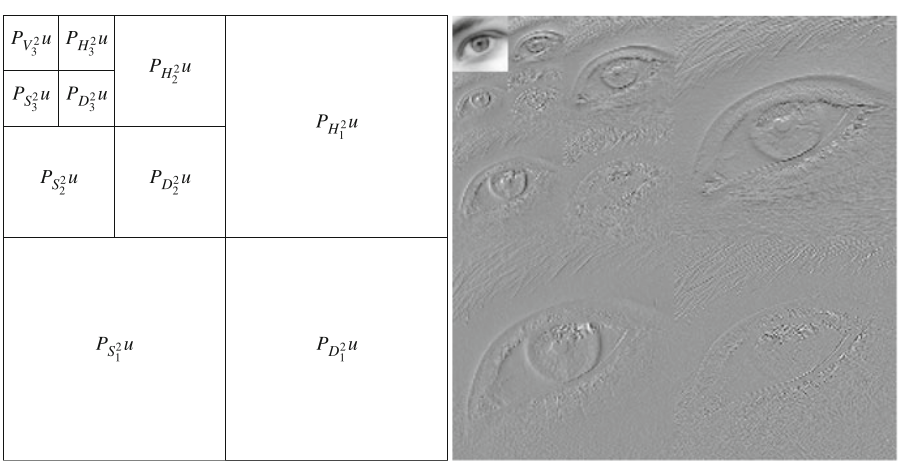
\includegraphics[scale=0.5]{wav.png}  %el parámetro scale permite agrandar o achicar la imagen. En el nombre de archivo puede especificar directorios
	\caption{La transformada wavelet discreta 2D de una imagen a través de la wavelet Haar} 
	\label{fig:wav}
\end{figure}

Este tipo de análisis multiescala bidimensional es fácil de implementar algorítmicamente: basado en la aproximación de los coeficientes $c^j$, calculamos los coeficientes $c^{j+1}$ es una escala mayor además de los tres coeficientes de detalles $d^{1,j+1}, d^{2,j+1}, d^{3,j+1}$. En la práctica, esto se consigue con la concatenación de la descomposición wavelet unidimensional a lo largo de las columnas y las filas:

\begin{figure}[H] %con el [H] le obligamos a situar aquí la figura
	\centering
	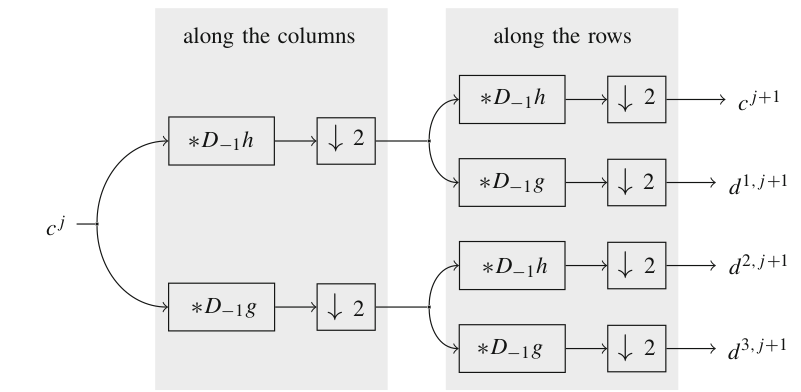
\includegraphics[scale=0.5]{esquema.png}  %el parámetro scale permite agrandar o achicar la imagen. En el nombre de archivo puede especificar directorios
	\caption{Esquema de actuación algorítmica para calcular transformada 2D} 
	\label{fig:esquema}
\end{figure}
\end{itemize}

\newpage

\subsubsection{Selección de características}

Una vez que hemos aplicado la transformada discreta wavelet 2D sobre cada una de los slices y hemos configurado nuestro dataset, nos encontramos con un conjunto de datos de enormes dimensiones, repleto de información (gran parte, probablemente, redundante o inútil en nuestro proyecto) que necesita ser estudiada. Esta basta cantidad de datos tiene dos grandes inconvenientes. El primero de ellos es que los algoritmos de aprendizaje no serán capaces de encontrar las características determinantes a la hora de clasificar instancias debido al gran ruido que tenemos (efecto Hughes). Por su parte, el segundo es un problema pragmático: los clasificadores no van a tener un rendimiento adecuado y tardarán demasiado tiempo en ejecutarse. Por tanto, es necesaria una selección de las características más importantes para así garantizar un mejor rendimiento y unas conclusiones más certeras. Existen multitud de técnicas en estadística multivariante para reducir la dimensionalidad. De entre ellas destaca Análisis de Componentes Principales (PCA) y por ello la utilizamos. PCA es una herramienta eficiente para reducir la dimensionalidad de un dataset formado un gran número de variables correladas entre sí. El objetivo es transformar el conjunto de datos en uno nuevo constituido por las variables ordenadas según el grado de importancia o varianza de las mismas. Esta técnica tiene tres efectos:

\begin{itemize}
	\item Ortogonaliza las componentes de los vectores de entrada para que no tengan correlación entre ellas.
	\item Ordena el resultado de las componentes ortogonales de mayor a menor en variación o importancia.
	\item Elimina aquellas componentes que aportan menor variación.
\end{itemize}

Téngase en cuenta que los vectores de entrada deben estar normalizados con media cero y desviación típica uno antes de utilizar el algoritmo. La normalización se realiza tal y como se explicó en la sección anterior. \\

PCA encuentra una función a través de la cual incluye grandes cantidades de información en muestras analizadas. Sin embargo, como las funciones son combinaciones lineales de las características originales, es difícil (por no decir imposible) interpretar las variables resultantes de la transformación. Desde el punto de vista clínico, este hecho hace que el estudio pierda valor médico, aunque es realmente necesario debido al volumen de datos que tenemos. De manera intuitiva, dado un espacio de características n-dimensional, PCA ajusta un elipsoide de la misma dimensión que contiene un porcentaje prefijado de la varianza de los datos y cada eje se convierte en una componente principal, por lo que si un eje es pequeño, su varianza también lo será. \\

Desarrollo ahora el contenido matemático de Análisis de Componentes Principales (\cite{amsa}, \cite{ms}).
\newpage
	
	Un vector aleatorio es un vector cuyas componentes son variables aleatorias. Por tanto, la media del vector es un vector formado por las medias de cada componente. Si $X = (X_1,\dots,X_n)$ es un vector aleatorio y $\mu = (\mu_1,\dots,\mu_n)$ es su vector media, entonces
	
	$$\mu_i = E(X_i) \hspace{0.5cm} i =1, \dots, n$$
	
	Sin embargo, la analogía para la varianza no es tan obvia. Definimos $var(X)$ como una matriz donde, para cada $i,j$, el elemento es $cov(X_i,X_j)$. Esto es lo que se llama la matriz de covarianzas de $X$. Esta matriz es siempre simétrica. \\
	
	Si $X$ e $Y$ son variables aleatorias e $Y$ es una función lineal de $X$, esto es, $Y = aX + b$ para alguna constante $a$ y $b$, entonces
	
	$$E(Y) = a E(X) + b$$
	$$var(Y) = a^2 var(X)$$
	$$\sigma(Y) =  |a| \sigma(X)$$
	
	Si $X,Y$ son vectores aleatorios, entonces decimos que $Y$ es una función lineal (afín) de $X$ cuando $Y = AX +b$, para alguna matriz constante $A$ y algún vector constante $b$. Tenemos que
	
	$$E(Y) = A E(X) + b $$
	$$var(Y) = A var(X) A^T$$
	
	
	Consideremos el caso en que $Y = AX$, siendo $A$ una matriz fila. Por tanto, $AX$ es un escalar. Por convención, $A = a^T$, siendo $a$ un vector columna. De la igualdad anterior tenemos que
	
	$$ 0 \leq var(Y) = a^T var(X) a$$
	
	teniendo en cuenta que la varianza de una variable aleatoria siempre es no negativa. Esta propiedad tiene un nombre. Un matriz simétrica $V$ se dice que es semi-definida positiva si 
	$$a^T V a \geq 0 \hspace{1cm} \forall a$$
	
	Por tanto, la matriz de covarianzas es simétrica y semi-definida positiva. \\
	
	Tratamos ahora la descomposición espectral. Toda matriz simétrica tiene una descomposición espectral
	
	$$A = ODO^T$$
	donde $D$ es diagonal y $O$ una matriz ortogonal. Pensando en $O$ como un cambio de sistema de coordenadas, encontramos una correspondencia con los movimientos rígidos (rotaciones) con ejes coordenados perpendiculares. La descomposición espectral puede utilizarse para determinar si una matriz es semi-definida positiva. 
	
	\textbf{Proposición.} Una matriz diagonal es semi-definida positiva si y solamente si todos sus elementos son no negativos.
	
	\textbf{Demostración} Basta ver que 
	$$a^T D a = \sum_{i} a_i^2 d_ii.$$
	\hfill$\blacksquare$
	
	En general, una matriz simétrica es semi-definida positiva si y solamente si la matriz diagonal de su descomposición espectral es semi-definida positiva, ya que
	
	$$a^T A a = a^T ODO a = b^t D b$$
	
	donde $b= O^Ta$ y $a = Ob$. \\
	
	Tratamos ahora los valores y vectores propios. Multiplicando a la derecha por $O$, tenemos que
	
	$$AO = ODO^TO = OD$$
	
	Si observamos este resultado por columnas $w_i \in O$, tenemos que
	$$ A w_i = \lambda_i w_i$$
	
	donde $\lambda_i$ es el i-ésimo elemento de $D$.
	
	Por tanto, los elementos de $D$ son los valores propios de $A$ y las columnas de $O$, sus correspondientes vectores propios. \\
	
	Una vez introducidos estos sencillos conceptos, nos adentramos en Componentes Principales. Si $X$ es un vector aleatorio de varianza finita, sea 
	$$var(X) = ODO^T$$
	la descomposición espectral de su matriz de covarianzas.
	
	Considero el vector aleatorio $Y = O^T X$. Entonces
	
	$$var(Y) = O^T var(X) O = O^T ODO^T O = D$$
	
	ya que $O$ es ortogonal. Por tanto, $Y$ tiene una matriz de covarianzas diagonal. Por tanto, como los elementos que están fuera de la diagonal de la matriz de covarianzas son las propias covarianzas de las variables, las componentes de $Y$ no están correladas. Y ya que los elementos de la diagonal de la matriz de covarianzas son la varianza de cada variable y los elementos de $D$ son los valores propios de $var(X)$, las varianzas de los componentes de $Y$ son los valores propios de la matriz de covarianzas de $X$. \\
	
	Los elementos de $Y$ son las llamadas componentes principales de $X$. Dado que una matriz ortogonal es invertible, tenemos que $X = OY$. Esto expresa una variable aleatoria cualquiera como una combinación lineal de variables aleatorias independientes. Este proceso de  hacer la descomposición espectral de la matriz de covarianzas de X es el llamado Análisis de Componentes Principales.
	
	PCA se usa como método de reducción de dimensionalidad. Si tomamos unos pocos componentes principales, obtenemos una explicación simple de la estructura de $X$ a través de unas pocas variables.Deben ordenarse las componentes de $Y$ poniendo en primer lugar las componentes más grandes (los mayores valores propios). Por último, tratamos la varianza explicada. Sea $\Vert · \Vert$ la norma Euclídea de un vector, por lo que
	
	$$ \Vert Y \Vert^2 = Y^T Y = \sum_{i} Y_i^2$$
	
	Como las componentes de $Y$ son independientes, tenemos que 
	
	$$E(\Vert Y - v \Vert^2) = \sum_{i=1}^{n} \lambda_i$$
	
	donde $v = E(Y)$. Dado que una transformación ortogonal es una rotación (isometría), no afecta a distancias ni longitudes. Si $\mu = E(X)$, tenemos
	
	$$E(\Vert X -\mu \Vert^2) = E((X-\mu)^T (X-\mu)$$
	$$ = E((Y-v)^T O^T (Y-v)$$
	$$ = E((Y-v)^T (Y-v)) $$
	$$E(\Vert Y-v \Vert^2)$$
	
	Dado que $Y = O^TX$, $X = OY$ y $\mu = O v$. De forma similar, si $\overline{\mu} = E(\overline{X})$, entonces
	
	$$E(\Vert \overline{X}- \overline{\mu} \Vert^2) = \sum_{i=1}^{k} \lambda_i$$
	
	La fracción de varianza de $X$ explicada por las primeras $k$ componentes principales es
	$$\frac{\sum_{i=1}^{k} \lambda_i}{\sum_{i=1}^{n} \lambda_i}$$
	

En nuestro proyecto, utilizamos siempre PCA con una varianza explicada del 95\%.
\newpage
\subsection{Clasificación}

En esta sección expongo los distintos algoritmos que hemos usado para clasificar a los sujetos según las imágenes MRI. El primero de ellos será SVM. Más tarde, nos enfrentaremos a la necesidad de ajustar los hiperparámetros del modelo optimizando así los resultados. De igual manera, nos enfrentaremos al problema del sobre ajuste, que solucionamos con Validación Cruzada de 10 particiones. Será necesaria también la mención de las redes neuronales profundas y, finalmente, la regresión logística.

\subsubsection{SVM}

SVM es un clasificador (aprendizaje supervisado) muy potente introducido en 1995. Consigue resultados buenos en clasificación especialmente en diagnóstico médico. SVM se basa en el principio de minimización del riesgo estructural proveniente de la teoría del aprendizaje en estadística. Su objetivo es encontrar un hiperplano separador óptimo entre los miembros y los no miembros de una clase en un espacio de características de varias dimensiones. La entrada al algoritmo está formada por un subconjunto de características elegidas por medio de la extracción y selección de las mismas. En nuestro caso, las clases son Control (sano) y PD (enfermo de PD), por lo que dividir los pacientes sigue siendo nuestro objetivo. Veamos su fundamentación matemática (\cite{esl}): \\

Supongamos que disponemos de un conjunto de instancias divididas en dos clases linealmente separables. Nuestro conjunto de entrenamiento está formado por $N$ parejas $(x_1,y_1),(x_2,y_2),\dots (x_n,y_n)$ con $x_i \in \mathbb{R}^p, y_i \in \{1,-1\}$. Definimos el hiperplano

$$\{x:f(x) = x^T \beta + \beta_0 = 0 \}$$

donde $\beta$ es un vector unitario. La función que clasifica inducida por $f(x)$ es 

$$G(x) = sign[x^T \beta + \beta_0]$$


Esta última expresión representa la distancia con signo de un punto $x$ al hiperplano $f(x) = x^T \beta + \beta_0=0$. Dado que las clases son separables, podemos encontrar una solución $f(x) = x^T \beta + \beta_0$ con $y_if(x_i) > 0 \forall i$. En consecuencia, somos capaces de encontrar un hiperplano que genera el mayor \textit{margen} entre las instancias de entrenamiento para las clases 1 y -1 (Figura 3.7)

\begin{figure}[H] %con el [H] le obligamos a situar aquí la figura
	\centering
	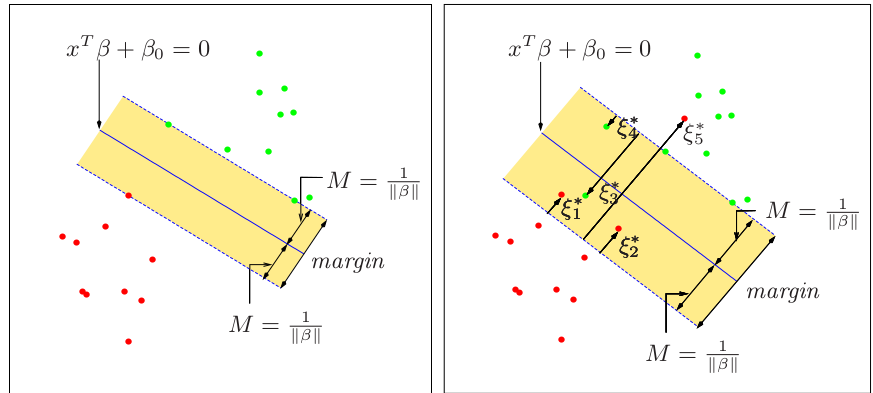
\includegraphics[scale=0.5]{hip.png}  %el parámetro scale permite agrandar o achicar la imagen. En el nombre de archivo puede especificar directorios
	\caption{Hiperplano separador con el margen y los vectores soporte (aquellos que definen la región)} 
	\label{fig:hip}
\end{figure}

El problema de optimización es el siguiente: 
$$max_{\beta, \beta_0, \Vert \beta \Vert = 1} M$$
$$\text{sujeto a } y_i(x_i^T\beta + \beta_0) \geq M, i=1,\dots,N$$

La banda tiene una anchura de $2M$ ($M = \frac{1}{\beta}$ desde cada clase) y se llama margen. Por la definición de $M$, es posible reformular el problema de una forma más sencilla

$$min{\beta, \beta_0} \beta$$
$$\text{sujeto a } y_i(x_i^T\beta + \beta_0) \geq M, i=1,\dots,N$$

Este es un problema de optimización con funciones convexas que se resuelve con los procedimientos clásicos del análisis real de varias variables. \\

Supongamos ahora que las clases se solapan en el espacio de características. Una forma de enfrentarnos a ese solapamiento es maximizar $M$ permitiendo a algunos puntos estar mal clasificados (quedarse en el lado erróneo del margen). Si definimos esa anomalía a a través de una variable $\xi = (\xi_1,\dots,\xi_n)$, podemos representar el problema de restricciones anterior de la siguiente manera

$$y_i(x_i^T\beta+\beta_0) \geq M(1-\xi_i)$$
$\forall i, \xi_i \geq 0, \sum_{i=1}^{N} \xi_i \leq cte$.

La idea es la siguiente. El valor $\xi_i$ en la restricción $y_i(x_i^T\beta+\beta_0) \geq M(1-\xi_i)$ es la cantidad proporcional por la que la predicción $f(x_i) = x_i^T \beta + \beta_0$ está en el lado erróneo del margen. Por tanto, acotando $\sum \xi_i$, acotamos la cantidad proporcional total a las predicciones mal situadas. Estos errores en la clasificación ocurren cuando $\xi_i > 1$, así que acotar $\sum \xi_i$ por una constante $K$ acota superiormente el número de instancias mal clasificadas por $K$.

Como antes, podemos eliminar la restricción sobre la norma de $\beta$, ya que $M = \frac{1}{\Vert \beta \Vert}$ y escribimos

$$min \Vert \beta \Vert$$
$$\text{sujeto a } y_i(x_i^T \beta + \beta_0) \geq 1-\xi_i \forall i \text{  y  } \xi_i \geq 0, \sum \xi_i \leq cte.$$ 

\begin{figure}[H] %con el [H] le obligamos a situar aquí la figura
	\centering
	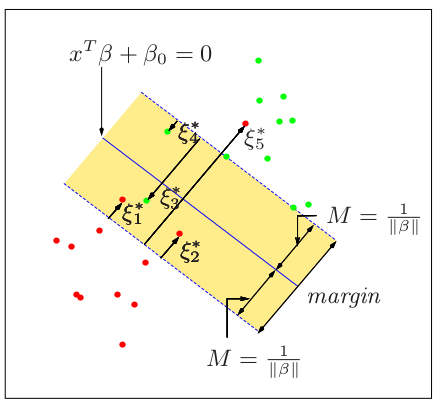
\includegraphics[scale=0.5]{hip2.png}  %el parámetro scale permite agrandar o achicar la imagen. En el nombre de archivo puede especificar directorios
	\caption{Hiperplano separador con el margen y clases solapadas} 
	\label{fig:hip2}
\end{figure}

El problema anterior es cuadrático con inecuaciones lineales como restricciones, luego es un problema de optimización convexo. Para resolverlo, utilizamos los multiplicadores de Lagrange. Reescribimos la expresión de una forma más conveniente desde el punto de vista computacional

$$min_{\beta,\beta_0} \frac{1}{2} \Vert \beta \Vert^2 + C \sum_{i=1}^{N} \xi_i$$
$$\text{sujeto a } \xi_i \geq 0, y_i(x_i^T \beta + \beta_0) \geq 1- \xi_i \forall i$$

donde $C$ es un parámetro que refleja el coste (para un problema donde es linealmente separable, $C= \infty$).

El lagrangiano es

$$L_p = \frac{1}{2} \Vert \beta \Vert^2 + C \sum_{i=1}^{N} \xi_i - \sum_{i=1}^{N}\alpha_i[y_i(x_i^T \beta + \beta_0)-(1-\xi_i)] - \sum_{i=1}^{N} \mu_i \xi_i$$

en la que minimizamos respecto de $\beta, \beta_0$ y $\xi_i$. Derivando e igualando a cero obtenemos

$$\beta = \sum_{i=1}^{N} \alpha_i y_i x_i,$$
$$0 = \sum_{i=1}^{N} \alpha_i y_i$$
$$\alpha_i = C-\mu_i \forall i$$

además de las restricciones $\alpha_i,\mu_i,\xi_i \geq 0 \forall i$. Sustituyendo en la expresión anterior, obtenemos que

$$L_D = \sum_{i=1}^{N}\alpha_i - \frac{1}{2}\sum_{i=1}^{N}\sum_{i'=1}^{N}\alpha_i \alpha_{i'} y_i y_{i'}x_i^T x_{i'}^T$$

Ahora, maximizamos $L_D$ sujeto a que $0 \leq \alpha_i \leq C$ y $\sum_{i=1}^{N} \alpha_i y_i=0$. Además de las ya presentadas, las condiciones de Karush-Kuhn-Tucker (\cite{kkt}) incluyen las restricciones

$$\alpha_i[y_i(x_i^T \beta + \beta_0)-(1-\xi_i)] = 0$$
$$\mu_i \xi_i = 0$$
$$y_i(x_i^T \beta + \beta_0)-(1-\xi_i) \geq 0$$

para $i = 1,\dots, N$\\

De la igualdad correspondiente a $\beta$, vemos que la única solución tiene la forma

$$\hat{\beta} = \sum_{i=1}^{N} \hat{\alpha_i} y_i x_i$$

para coeficientes $\hat{\alpha_i}$ distintos de cero que cumplen las restricciones citadas. Estas observaciones son los llamados vectores soporte. \\ 

\textbf{SVM y núcleos}\\

El clasificador descrito hasta ahora encuentra los bordes de los datos en el espacio de características de forma lineal. Podemos hacer este procedimiento más flexible aumentando el espacio de características usando extensiones basadas en polinomios o splines. Generalmente, los bordes lineales consiguen una mejor separación entre las clases del conjunto de entrenamiento en espacio mayores y se traducen en bordes no lineales en el espacio original. Una vez que las funciones base $h_m(x), m=1,\dots,M$ han sido seleccionadas, el procedimiento es igual que antes. Ajustamos el clasificador usando las características $h(x_i) = (h_1(x_i),\dots,h_M(x_i)), i = 1, \dots, N$ y producimos la función (no lineal) $\hat{f}(x) = h(x)^T \hat{\beta} + \hat{\beta_0}$. El target finalmente es, como antes,  $\hat{G}(x)= sign(\hat{f}(x))$. Utilicemos esta idea para extender el concepto de SVM. Si escribimos la función lagrangiana dual 

$$L_D = \sum_{i=1}^{N}\alpha_i - \frac{1}{2}\sum_{i=1}^{N}\sum_{i'=1}^{N}\alpha_i \alpha_{i'} y_i y_{i'}\langle h(x_i),h(x_{i'})\rangle$$

y utilizando la expresión de $f$, tenemos que

$$f(x) = h(x)^T \beta + \beta_0$$
$$= \sum_{i=1}^{N} \alpha_i y_i \langle h(x),h(x_i) \rangle + \beta_0$$

Como antes, dado $\alpha_i, \beta_0$ puede calcularse por medio de la ecuación $$ y_i f(x_i) = 1$$ $\forall x_i \text{ con } 0 < \alpha_i < C$.

Las dos expresiones anteriores involucran a $h$ a través de productos escalares. En realidad, no necesitamos conocer $h$ si no el núcleo

$$K(x,x) = \langle h(x),h(x') \rangle$$

que calcula los productos escalares en los espacios transformados. $K$ debe ser simétrica y semidefinida positiva. Existen tres núcleos popularmente utilizados en la literatura:
\begin{itemize}
		\item Polinomial de grado $d$: $K(x,x') = (1+\langle x,x'\rangle) ^d$
		\item Base radial: $K(x,x') = exp(-\gamma \Vert x-x'\Vert^2)$
		\item Red neuronal: $K(x,x') = tanh(k_1 \langle x, x' \rangle + k_2)$
\end{itemize}

Finalmente, la solución tiene la expresión

$$\hat{f}(x) = \sum_{i=1}^{N} \hat{\alpha_i}y_i K(x,x_i)+\hat{\beta_0}$$

\subsubsection{Validación cruzada con K-particiones}

Validación cruzada es una técnica de validación de modelos que determina la robustez de los resultados de nuestro análisis estadístico. De forma específica, hace más robusta la fase de entrenamiento haciendo particiones k sucesivas, a su vez,de entrenamiento y validación, de forma que k-1 partes quedan para entrenar y una para testear el modelo. El proceso es llevado a cabo k veces reduciendo así la variabilidad. En nuestro proyecto utilizamos 10 particiones.

\begin{figure}[H] %con el [H] le obligamos a situar aquí la figura
	\centering
	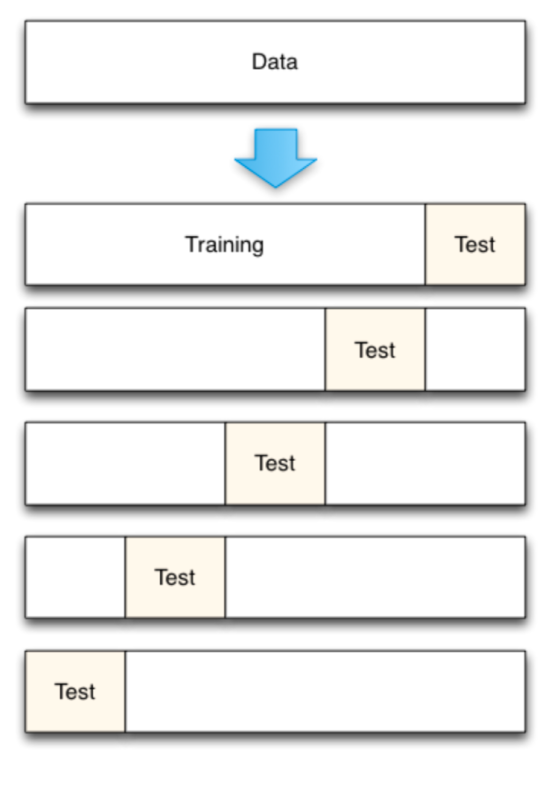
\includegraphics[scale=0.5]{cv.png}  %el parámetro scale permite agrandar o achicar la imagen. En el nombre de archivo puede especificar directorios
	\caption{Ejemplo de validación cruzada} 
	\label{fig:cv}
\end{figure}

\subsubsection{Ajuste de hiperparámetros y GridSearch}

Mientras ejecutamos la validación cruzada de 10 particiones intentamos encontrar los mejores parámetros $C$ y $\gamma$ a través de un grid search. Grid Search es una técnica utilizada para la optimización de hiperparámetros, asegurando así que los modelos no sobre ajustan. Este proceso consiste en una búsqueda exhaustiva en un rango definido para la pareja $(C,\gamma)$. Aquella pareja que consiga el mayor \textit{recall} (\textit{accuracy} no es la mejor medida en biomedicina, puesto que lo que queremos evitar son los falsos negativos) es seleccionada para el training. Los rangos de valores son los siguientes:
\begin{itemize}
	\item $C = \{2^{i},i=-2,\dots,11\} $
	\item $\gamma = \{2^{i}, i =-9,\dots,3\}$
\end{itemize}

\subsubsection{Regresión logística}

La última pieza de nuestro clasificador, antes de explicar la arquitectura completa, es la regresión logística (\cite{esl}). Los modelos de regresión logística surgen por el deseo de modelar la probabilidad a posteriori de las $K$ clases a través de una función lineal en $x$, mientras que al mismo tiempo se aseguran de que suman 1 y se mantienen en el intervalo [0,1] (es una probabilidad). el modelo tiene la forma

$$\log \frac{P(G=1| X =x)}{P(G=K|X=x} =  \beta_{10} + \beta_1^Tx$$
 $$\log \frac{P(G=2| X =x)}{P(G=K|X=x} =  \beta_{20} + \beta_2^Tx$$
 $$\vdots$$
 $$\log \frac{P(G=K-1| X =x)}{P(G=K|X=x} =  \beta_{(K-1)0} + \beta_{K-1}^Tx$$
 
 A pesar de que el modelo utiliza la última clase en el denominador de cada expresión, la elección de dicho denominador es arbitraria y la estimaciones son invariantes bajo esta elección. Un simple cálculo muestra que
 
 $$P(G=k| X=x) = \frac{exp(\beta_{k0}+\beta_k^T x)}{1+\sum_{l=1}^{K-1}exp(\beta_{l0}+\beta_l^Tx)}$$
  $$P(G=K| X=x) = \frac{1}{1+\sum_{l=1}^{K-1}exp(\beta_{l0}+\beta_l^Tx)}$$
  
  con $k=1,\dots,K-1$ y claramente suman 1. Para enfatizar la dependencia sobre el conjunto de parámetros $\theta = {\beta_{10},\beta_1^T,\dots,\beta_{(K-1)0},\beta_{K-1}^T}$, denotamos las probabilidades $P(G=k|X=x) = p_k(x;\theta)$. \\
  
  Cuando $K=2$ (nuestro caso), el modelo especialmente simple, ya que se trata exclusivamente de una función lineal. \\
  
  \textbf{Ajustando un modelo de regresión logística} \\
  
  Los modelos de regresión logística se ajustan habitualmente con el principio de máxima verosimilitud, usando la verosimilitud condicionada a G dado X. Dado que P(G|X) especifica completamente la distribución condicional, la utilización de la multinomial es adecuada. La \textit{log-verosimilitud} para $N$ observaciones es
  
  $$l(\theta) = \sum_{i=1}^{N} \log p_{g_i}(x_i;\theta)$$
  donde $p_k(x_i;\theta) = P(G=k|X=x_i)$. Nos centramos en $K=2$, puesto es el caso que nos ocupa. Supongamos que las dos clases que tenemos se codifican como 0/1, de forma que $y_i=1$ cuando $g_i=1$ y $y_i=0$ cuando $g_i=2$. Sea $p_1(x;\theta) = p(x;\theta), p_2(x;\theta) = 1 -p(x;\theta)$. La \textit{log-verosimilitud} se puede escribir como
  
  $$l(\beta) = \sum_{i=1}^{N} \{ y_i \log p(x_i;\beta)+(1-y_i) \log(1-p(x_i;\beta)) \}$$
  $$ = \sum_{i=1}^{N} \{y_i \beta^T x_i - \log(1+e^{\beta^T x_i}) \}$$
  
  Aquí, $\beta = \{\beta_{10},\beta_1 \}$ y asumimos que el vector de entrada $x_i$ incluye el término constante 1. Para maximizar la \textit{log-verosimilitud}, derivamos e igualamos a cero:
  
  $$\frac{\partial l(\beta)}{\partial \beta} = \sum_{i=1}^{N} x_i (y_i -p(x_i;\beta))=0$$
  
  siendo $p+1$ ecuaciones no lineales en $\beta$.  Para resolverlas utilizamos el algoritmo de Newton-Raphson, que requiere el cálculo de la matriz Hessiana
  
  $$\frac{\partial^2 l(\beta)}{\partial \beta \partial \beta^T} = - \sum_{i=1}^{N} x_i x_i^T p(x_i;\beta)(1-p(x_i;\beta))$$
  
  Empezando con un $\beta^{old}$, tenemos que
  
  $$\beta^{new} = \beta^{old} - \left(\frac{\partial^2 l(\beta)}{\partial \beta \partial \beta^T}\right)^2 \frac{\partial l(\beta)}{\partial \beta}$$
  
  donde las derivadas se evalúan en $\beta^{old}$. Escribimos nuestras ecuaciones en forma matricial, de forma que $\textbf{y}$ es el vector que contiene a las $y_i$, $\textbf{X}$, de $N \times (p+1)$ la matriz de $x_i$, $\textbf{p}$   el vector de probabilidades $p(x_i;\beta^{old})$ y $\textbf{W}$ una matriz diagonal $N \times N$ con los pesos $p(x_i;\beta^{old})(1-p(x_i;\beta^{old}))$. Así, tenemos
  
  $$\frac{\partial l(\beta)}{\partial \beta} = X^T(y-p)$$
  $$\frac{\partial^2 l(\beta)}{\partial \beta \partial \beta^T} = -X^TWX$$
  
  y por tanto, los pasos del método de Newton son
  
  $$\beta^{new} = \beta^{old} + (X^TWX)^{-1}X^T(y-p)$$
  $$ = (X^TWX)^{-1} X^T W(X \beta^{old}+W^{-1}(y-p))$$
  $$ = (X^TWX)^{-1} X^T Wz$$
  
  Parece que $\beta = 0$ es un buen punto de inicio para el proceso iterativo, aunque la convergencia nunca está garantizada. Generalmente el algoritmo converge, ya que la \textit{log-verosimilitud} es cóncava.
  
\subsubsection{Optimización: En busca de los mejores cortes}

Una vez explicadas las principales herramientas dentro de la clasificación, es momento de conectarlas y darles sentido. Nuestro objetivo es encontrar aquellos cortes (\textit{slices}) que nos dan la información más veraz a la hora de diagnosticar la enfermedad del Parkinson. En trabajos anteriores como  \cite{irojas} o \cite{alberto}  se utilizó un algoritmo genético como optimización (NSGA-II). Yo propongo una alternativa que considero más eficiente desde un punto de vista computacional. Mi idea nace en el seno de los llamados \textit{ensemble learner}. En particular, utilizo \textit{stacking} de la siguiente manera. En una primera fase, utilizando solamente los 189 cortes del plano Coronal (se explicará en la siguiente sección por qué) genero 189 clasificadores, uno por slice, de manera que cada  paciente pasa por todos ellos (en su slice correspondiente, especializándose en ella), aprende las características propias de las mismas y genera una predicción sobre el conjunto de test. Así, cuando se han completado los 189 procesos, contamos con un dataset nuevo repleto de las predicciones generadas por los modelos, de forma que cada fila es un paciente y cada columna un slice (por lo que la dimensión es $Num\_pacientes \times 189$). Aquí interviene la segunda parte del \textit{stacking}, en la que empleo un modelo lineal (regresión logística) para calcular los pesos de cada slice, viendo cuál es la que tiene más transcendencia a la hora de clasificar un paciente como enfermo o sano. En cada una de las fases, separo los datos en train y test, llevando a cabo una validación cruzada. 

\begin{figure}[H] %con el [H] le obligamos a situar aquí la figura
	\centering
	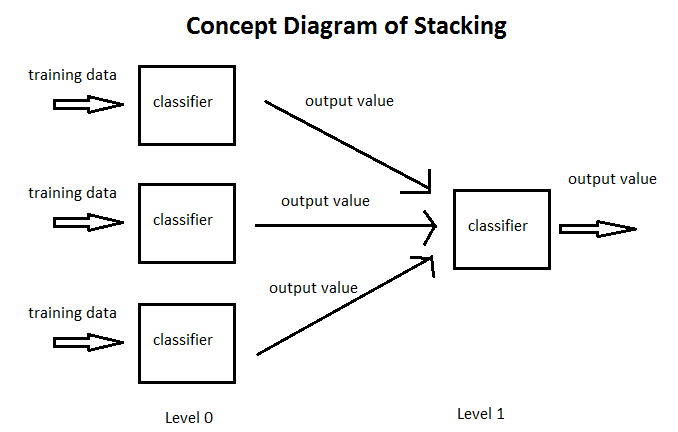
\includegraphics[scale=0.5]{stacking.png}  %el parámetro scale permite agrandar o achicar la imagen. En el nombre de archivo puede especificar directorios
	\caption{Modelo de stacking} 
	\label{fig:stack}
\end{figure}

\subsubsection{Deep Learning y Stacking}

Antes de describir con detalle la herramienta de deep learning que he utilizado, las Redes Neuronales Convolucionadas (CNN), introduzco qué es una Red Neuronal. Para su estudio, he realizado los cursos \cite{curso-cnn}, \cite{curso-nn}, consultas en  \cite{miriam} y he seguido de forma fidedigna el libro \cite{berzal}.

\begin{itemize}
	\item \textbf{REDES NEURONALES}
	
	Una Red Neuronal es un sistema computacional que trata de imitar o aproximar la sinapsis que se produce entre las neuronas del cerebro humano. Matemáticamente hablando, podemos decir que estos sistemas tratan de aproximar funciones dados unos input (de hecho, son aproximadores universales). Estas redes, al igual que un cerebro humano, están compuestas por neuronas. Cada neurona posee un peso, una función de activación y está conectada con otro conjunto de neuronas:
	
	\begin{figure}[H] %con el [H] le obligamos a situar aquí la figura
		\centering
		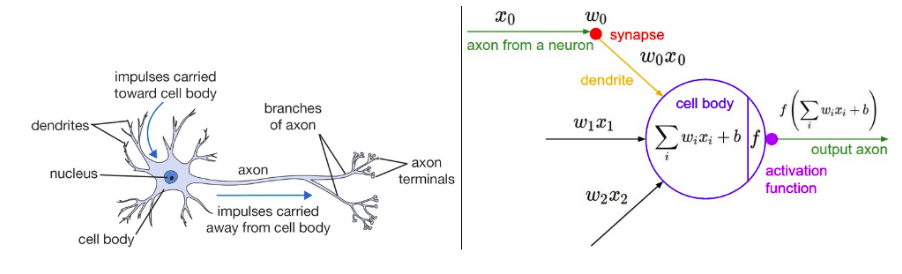
\includegraphics[scale=0.48]{nn1.png}  %el parámetro scale permite agrandar o achicar la imagen. En el nombre de archivo puede especificar directorios
		\caption{Comparación entre el cerebro humano y una red neuronal (\cite{miriam})} 
		\label{fig:nn1}
	\end{figure}
	
	Respecto de la topología de las redes y su conectividad, encontramos distintos casos en la literatura (\cite{berzal}):
	
	\begin{itemize}
		\item En cadena
		\item En cascada
		\item Con saltos
		\item Con múltiples cabezas
		\item Arquitecturas especializadas
	\end{itemize}
	
	Como ejemplos de funciones de activación, presento las más significativas (\cite{miriam}):
	
	\begin{enumerate}
		\item Función sigmoide $\sigma$, descrita por la curva $\sigma(x) = \frac{1}{1+e^{-x}}$, produciendo valores en el intervalo [0,1]. Son útiles para la última capa de la red para clasificaciones multi etiqueta.
		\item Función ReLu (\textit{Rectified Linear Unit}) cuya curva es $f(x) = max(0,x)$.
		\item Función \textit{Softmax}.  Normalmente interpretada como una distribución de probabilidad, tiene la siguiente expresión $\sigma(x)_i = \frac{e^{x_i}}{\sum_{k=1}^{K} e^{x_k}}$
			\end{enumerate}
		Las redes neuronales suelen tener una gran cantidad de capas. Aquellas que no son las de entrada y la salida se llaman capas ocultas, y sirven para aproximar funciones más complejas. 
		
		\begin{figure}[H] %con el [H] le obligamos a situar aquí la figura
			\centering
			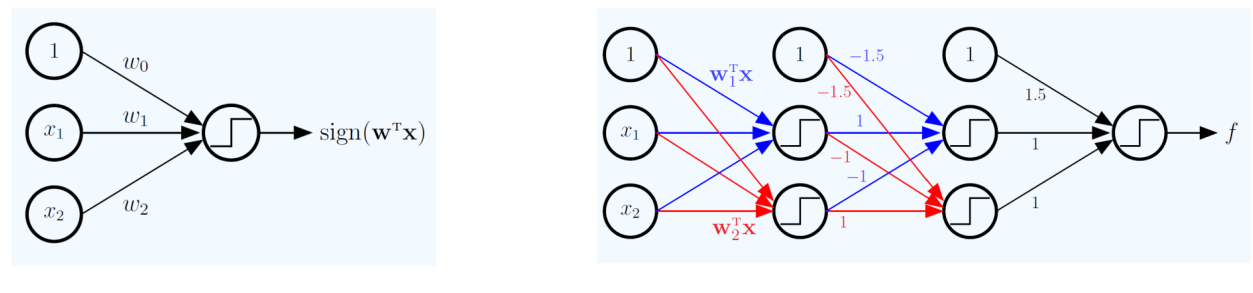
\includegraphics[scale=0.34]{nn2.png}  %el parámetro scale permite agrandar o achicar la imagen. En el nombre de archivo puede especificar directorios
			\caption{Ejemplo de red sencilla (izquierda) y red con capas ocultas (derecha) (\cite{esl})} 
			\label{fig:nn2}
		\end{figure}
	


\item \textbf{CNN} \\ \\
Una vez terminada la breve introducción sobre redes neuronales, nos introducimos en las redes neuronales convolutivas. Las redes convolutivas son las redes neuronales artificiales que se utilizan habitualmente para resolver múltiples problemas prácticos que requieren procesar imágenes. Por ejemplo, cuando la cámara frontal de un vehículo autónomo capta una señal de tráfico, debe identificar de qué señal concreta se trata. También puede interesarnos detectar qué tipo de objetos parecen en la imagen correspondiente a una escena y localizarlos dentro de la imagen (detección). Incluso podemos utilizar redes convolutivas como parte de un sistema que genera una descripción textual del contenido de una imagen, con lo que podemos indexar imágenes para realizar búsquedas por contenido en bases de datos de imágenes o sintetizar una señal de voz a partir de la descripción textual para usuarios invidentes. \\

¿En qué se diferencian las redes convolutivas de las redes multi capa presentadas antes? Principalmente, en que tanto sus entradas como sus salidas pueden ser estructuradas. Las redes convolutivas nos permitirán aprovechar dicha estructura para diseñar arquitecturas especializadas que resuelvan de un modo más eficiente problemas que trabajen con tipos particulares de señales. \\

En lugar de recibir un vector de entradas correspondientes a diferentes variables, recibiremos como entrada un vector, matriz o tensor en el que podemos explotar la relación física existente entre las diferentes entradas. EN el caso de señales unidimensionales, puede tratarse de una señal de audio en el que entradas adyacentes corresponden a muestras consecutivas en el tiempo. En el caso de señales bidimensionales, las entradas pueden corresponder a los píxeles de una imagen. También podemos tener señales bidimensionales de audio, como las provenientes de un array de micrófonos. En ocasiones, las señales de entrada puede que tengan más de dos dimensiones, como las imágenes en color, los datos volumétricos de imágenes médicas o un simple vídeo. \\

La salida de una red convolutiva puede ser convencional, para resolver problemas de clasificación usando una capa softmax (nuestro caso) o problemas de regresión. No obstante, habrá situaciones en las que su salida también reflejará la estructura de problemas que pretendemos resolver. Si trabajamos con imágenes, podemos construir una red convolutiva cuya salida también sea una imagen (\cite{berzal}). \\ \\

En lo siguiente, establecemos que nuestras entradas serán imágenes (slices del plano coronal). Estas redes tienen la particularidad de que las capas más cercanas a la imagen buscan características de bajo nivel, como es el caso de formas, texturas y colores. Mientras que las capas más cercanas a la salida buscan características semánticas de alto nivel, como personas, animales, tumores o deformaciones. Cabe destacar que basan su eficacia en la cantidad de capas dentro de su arquitectura (\cite{miriam}). Conforme crece el número de capas, el rendimiento mejora aunque aumenta, de igual manera, el coste computacional. \\

Situémonos en nuestro caso. Nuestras imágenes tienen unas dimensiones de 157x136x1= 21352 neuronas o pesos que debemos actualizar y propagar (el 1 es por estar en blanco y negro). Como se puede imaginar, el coste es brutal. Por ello, utilizamos capas especiales que palíen este defecto, como son las capas \textit{convolutional}, \textit{pooling} y \textit{dropout}.

\begin{itemize}
	\item Capas \textit{Convolutional} \\
	
	En ellas, cada neurona de una capa posterior cuenta con un rango de visión de la capa anterior, llamado campo local receptivo, de forma que las neuronas de la capa anterior que presenten una activación adecuada, contribuirán (a través de la convolución) a la entrada de la capa posterior. El ancho y alto del campo local receptivo  se denomina filtro y la cantidad de píxeles de la ventana se conoce como paso o stride. El objetivo es detectar una cierta característica en ventanas superpuestas y en distintas posiciones de la imagen. A las capas posteriores se les conoce como mapa de características. Después de cada convolución, se suele introducir una capa de activación ReLu.
	
	\item Capas \textit{Pooling} \\
	
	Debido a que la información generada por los mapas de características es ingente, es necesario resumirlos en una matriz que contenga la información más relevante. A este proceso se le llama Pooling. Cada neurona extraerá solamente el valor máximo o el valor medio de cada ventana (según el algoritmo) ignorando el resto. Así pues, el objetivo final de estas capas es reducir el número de pesos, evitando el sobre aprendizaje. \cite{miriam}
	
		\begin{figure}[H] %con el [H] le obligamos a situar aquí la figura
		\centering
		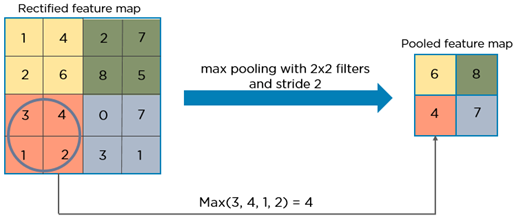
\includegraphics[scale=0.6]{pooling.png}  %el parámetro scale permite agrandar o achicar la imagen. En el nombre de archivo puede especificar directorios
		\caption{Ejemplo de pooling con máximo} 
		\label{fig:pooling}
	\end{figure}
	\vspace{2cm}
		\begin{figure}[H] %con el [H] le obligamos a situar aquí la figura
		\centering
		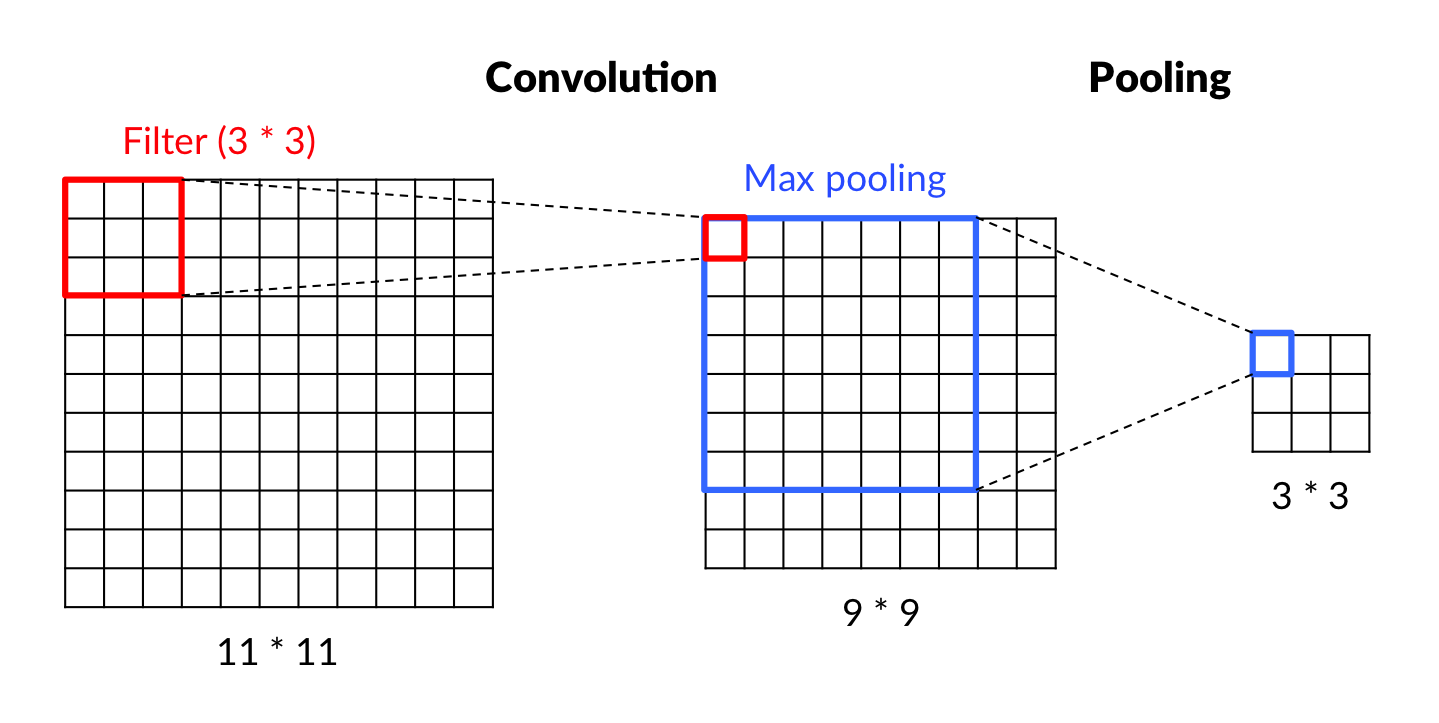
\includegraphics[scale=0.5]{conv-pool.png}  %el parámetro scale permite agrandar o achicar la imagen. En el nombre de archivo puede especificar directorios
		\caption{Ejemplo de convolución + pooling} 
		\label{fig:conv+pool}
	\end{figure}
	
\newpage	
	\item Capas \textit{Dropout} \\
	
	Una nueva medida para evitar el sobre ajuste. Se ``desconectan'' neuronas de forma aleatoria (llevar a cero un conjunto aleatorio de activaciones). 
						
		\begin{figure}[H] %con el [H] le obligamos a situar aquí la figura
		\centering
		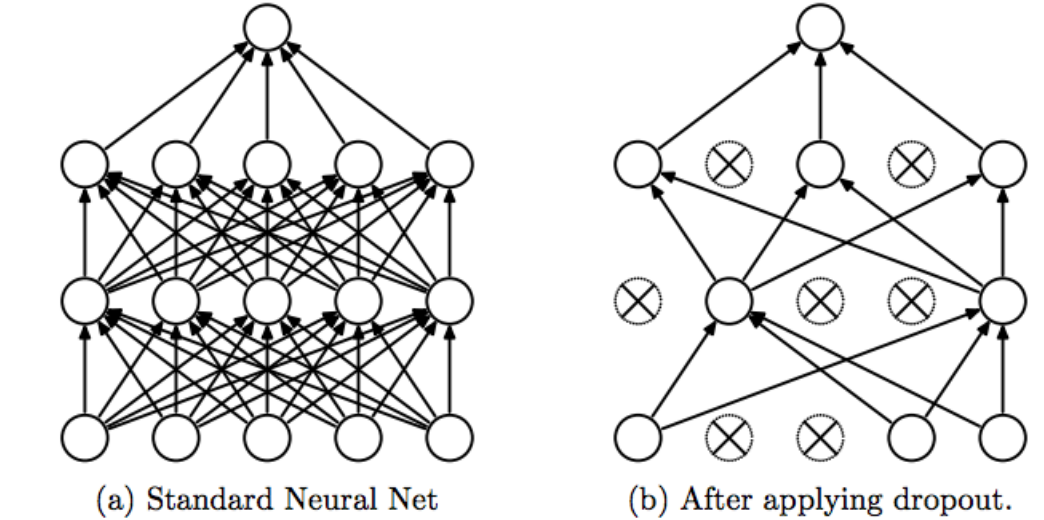
\includegraphics[scale=0.3]{dropout.png}  %el parámetro scale permite agrandar o achicar la imagen. En el nombre de archivo puede especificar directorios
		\caption{Ejemplo de dropout} 
		\label{fig:drop}
	\end{figure}				
\end{itemize}

 
\end{itemize}

Tras la introducción a redes neuronales y deep learning, relaciono la técnica \textit{stacking} con las redes profundas convolutivas. Mi voluntad es comparar los métodos de clasificación tradicionales (en este trabajo encarnados por SVM) con las redes, por lo que sustituiré SVM por CNN para completar la optimización en la búsqueda de las mejores slices. Todo ello será explicado con detenimiento en la siguiente sección.

\newpage 

\section{Metodología y experimentos}

En la presente sección desgloso los distintos experimentos realizados, explicando sus motivaciones y resultados principales. En resumen, estos han sido los experimentos:

\begin{itemize}
	\item El primer experimento consistió en decidir qué plano de las imágenes MRI es más importante para clasificar sujetos: X (Axial), Y (Coronal) o Z (Sagittal). Esto nos hizo reducir tiempo de cómputo y slices poco útiles.
	\item Tras decidir que plano utilizar, estudiamos el accuracy de cada slice y comparamos el rendimiento de la materia gris respecto al cerebro completo para mejorar el rendimiento de la clasificación.
	\item Primera optimización para los cortes más relevantes, en particular cortes del plano Coronal usando stacking y SVM.
	\item Segunda optimización con los mismos cortes usando stacking y CNN.
\end{itemize}

\newpage

\subsection{Experimento 1: Determinando el mejor plano}

En el experimento nos enfrentamos a la cuestión de qué plano dentro de una MRI es más representativo a la hora de clasificar a los pacientes, de forma que en lo sucesivo sólo utilizaremos este plano, ahorrando así tiempo de cómputo. \\

Usamos 100 pacientes en este experimento, 45 en el grupo de control y 55 enfermos de PD de la base de datos PPMI, normalizamos con la herramienta SPM de Matlab  y utilizamos SVM con el núcleo RBF.

\subsubsection{Material y metodología}

Las imágenes de los sujetos fueron, en primer lugar, segmentadas a través de la rutina de segmentación implementada en SPM12 (\cite{spm}). Tras ello, normalizamos y cambiamos el tamaño de la imagen a los bordes [-78 -112 -60; 78 76 85]. Extraemos características con la transformada discreta Wavelets 2D usando la transformada Bior3.3 hasta nivel 2. Tras ello, seleccionamos las características que explican el 95\% de la variabilidad en el conjunto de datos con PCA. Por último, el resultado de PCA fue ejecutado en SVM usando validación cruzada de 10 particiones y un conjunto de entrenamiento del 70\% de los datos. \\

Computamos los coeficientes wavelets 2D para cada slice y para cada paciente y llevamos a cabo la clasificación. Cada vez que entrenamos un SVM se realiza una permutación aleatoria de los pacientes para evitar el sesgo, de forma que el modelo no sobre ajusta, y realizamos 10 clasificaciones cada vez, quedándonos con la media de los resultados por cada slice. \\

Este proceso se lleva a cabo en cada uno de los planos de la imagen MRI: X,Y y Z. A continuación, presentamos los resultados.

\subsubsection{Resultados}

Queríamos comprobar qué plano tiene el mejor accuracy para así usarlo en los siguientes pasos. Analizamos los resultados de la clasificación para cada slice por separado. Llevamos a cabo esta prueba para cada tipo de plano, realizando la clasificación utilizando las mismas características en cada slice para cada sujeto.

\begin{figure}[H] %con el [H] le obligamos a situar aquí la figura
	\centering
	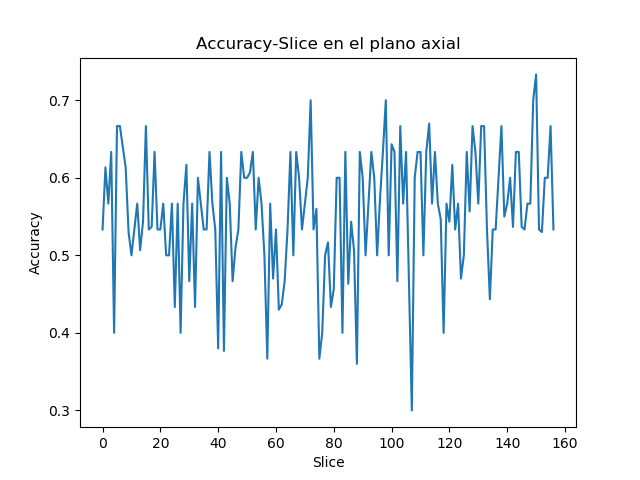
\includegraphics[scale=0.75]{exp1-axial.png}  %el parámetro scale permite agrandar o achicar la imagen. En el nombre de archivo puede especificar directorios
	\caption{Resultados para el plano axial} 
	\label{fig:exp1-axial}
\end{figure}

\begin{figure}[H] %con el [H] le obligamos a situar aquí la figura
	\centering
	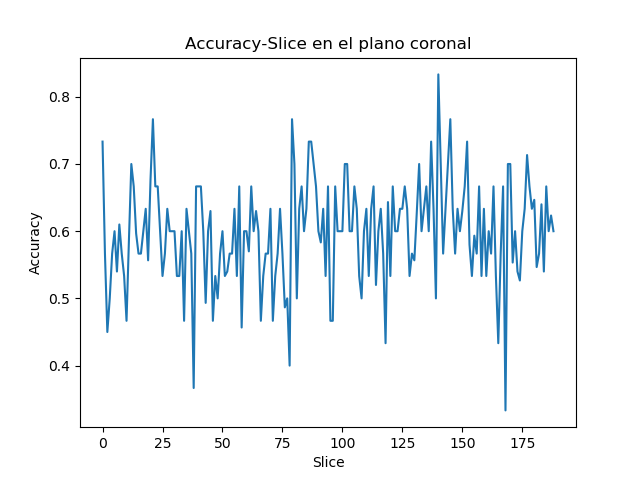
\includegraphics[scale=0.75]{exp1-cor.png}  %el parámetro scale permite agrandar o achicar la imagen. En el nombre de archivo puede especificar directorios
	\caption{Resultados para el plano coronal} 
	\label{fig:exp1-cor}
\end{figure}

\begin{figure}[H] %con el [H] le obligamos a situar aquí la figura
	\centering
	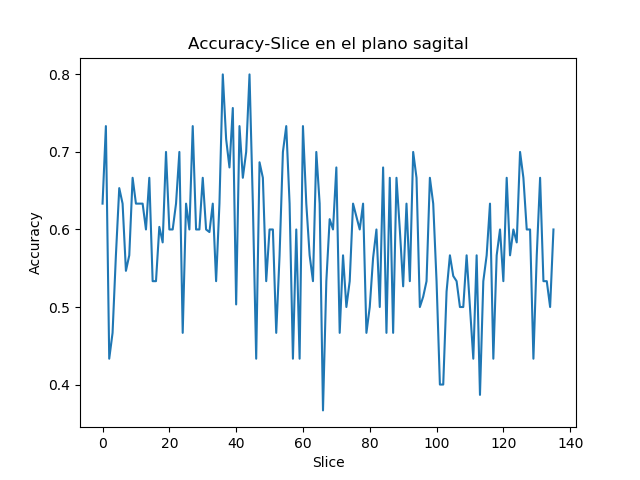
\includegraphics[scale=0.75]{exp1-sag.png}  %el parámetro scale permite agrandar o achicar la imagen. En el nombre de archivo puede especificar directorios
	\caption{Resultados para el plano sagittal} 
	\label{fig:exp1-sag}
\end{figure}

A primera vista no parece haber mucha diferencia entre las gráficas. Por tanto, he hecho un estudio más profundo contabilizando cuántas slices ``buenas'' (accuracy mayor del 75\%) hay para cada corte. Los resultados son los siguientes:

\begin{table}[H]
	\begin{tabular}{|c|c|c|c|c|c|}
		\hline
		& \textbf{\begin{tabular}[c]{@{}c@{}}Accuracy\\  medio\end{tabular}} & \textbf{\begin{tabular}[c]{@{}c@{}}Número \\ \\ de buenas\end{tabular}} & \textbf{\begin{tabular}[c]{@{}c@{}}Slices \\ \\ buenas\end{tabular}} & \textbf{Accuracy}                                                       & \textbf{\begin{tabular}[c]{@{}c@{}}Accuracy\\ Máximo\end{tabular}} \\ \hline
		\textbf{Axial}    & 0.5554140                                                          & 0                                                                       & -                                                                    & -                                                                       & \textless{}0.75                                                    \\ \hline
		\textbf{Coronal}  & 0.5974603                                                          & 4                                                                       & \begin{tabular}[c]{@{}c@{}}21,79,\\ 140,145\end{tabular}             & \begin{tabular}[c]{@{}c@{}}0.767,0.767, \\ \\ 0.833, 0.767\end{tabular} & 0.833                                                              \\ \hline
		\textbf{Sagittal} & 0.5866421                                                          & 3                                                                       & 36,39,44                                                             & 0.799, 0.756, 0.799                                                     & 0.799                                                              \\ \hline
	\end{tabular}
	\caption{Resultados del experimento 1}
\end{table}

Identificamos que el plano Coronal (Y) es el que tiene mayor accuracy medio y mayor número de slices con accuracy alto, por lo que lo utilizamos en el resto de experimentos.

\newpage 
\subsection{Experimento 2}

En este experimento, utilizamos 165 (65 del grupo de control y 100 enfermos de PD) imágenes MRI para estudiar cómo se comporta el rendimiento de clasificación utilizando sólo la información de la materia gris, de la materia blanca o del cerebro completo. Presentamos varias gráficas comparativas para cada tipo de imagen en cada corte del plano Coronal.

\subsubsection{Material y metodología}

Las imágenes de los sujetos fueron, en primer lugar, segmentadas a través de la rutina de segmentación implementada en SPM12 (\cite{spm}). Tras ello, normalizamos y cambiamos el tamaño de la imagen a los bordes [-78 -112 -60; 78 76 85]. Extraemos características con la transformada discreta Wavelets 2D usando la transformada Bior3.3 hasta nivel 2. Tras ello, seleccionamos las características que explican el 95\% de la variabilidad en el conjunto de datos con PCA. Por último, el resultado de PCA fue ejecutado en SVM usando validación cruzada de 10 particiones y un conjunto de entrenamiento del 70\% de los datos. \\

Computamos los coeficientes wavelets 2D para cada slice y para cada paciente y llevamos a cabo la clasificación. Cada vez que entrenamos un SVM se realiza una permutación aleatoria de los pacientes para evitar el sesgo, de forma que el modelo no sobre ajusta, y realizamos 10 clasificaciones cada vez, quedándonos con la media de los resultados por cada slice. \\

Llevamos a cabo este proceso para C1 (materia gris), C2 (materia blanca) y C1+C2 de las imágenes. 

\subsubsection{Resultados}

El objetivo de este experimento era comprobar qué tipo de información es más interesante para obtener el máximo accuracy en la clasificación. Además, descartar una parte de la imagen hace que el tiempo de cómputo general se reduzca mucho. \\

Presentamos los siguientes gráficos: En primer lugar, una imagen que muestra los resultados del accuracy para C1 y C2 superpuestos. A continuación, la diferencia de accuracy C2-C1 en cada slice (para ver la tendencia). Por último, presentamos el número de componentes principales para cada tipo de información.

\begin{figure}[H] %con el [H] le obligamos a situar aquí la figura
	\centering
	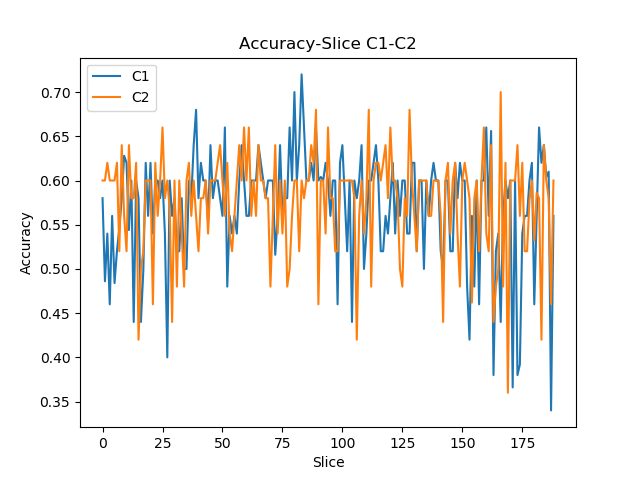
\includegraphics[scale=0.7]{accuracyc1c2.png}  %el parámetro scale permite agrandar o achicar la imagen. En el nombre de archivo puede especificar directorios
	\caption{Comparativa de accuracy entre C1 y C2} 
	\label{fig:comp-c1-c2}
\end{figure}

No vemos claramente qué tipo de información es más interesante. Veamos la diferencia:

\begin{figure}[H] %con el [H] le obligamos a situar aquí la figura
	\centering
	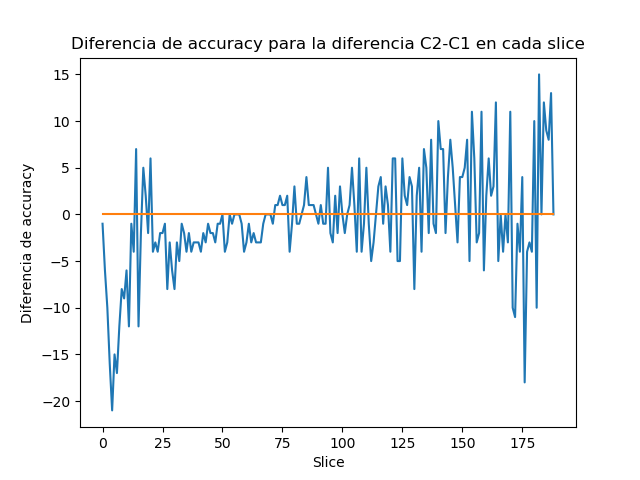
\includegraphics[scale=0.7]{C2-C1.png}  %el parámetro scale permite agrandar o achicar la imagen. En el nombre de archivo puede especificar directorios
	\caption{Diferencia de accuracy entre C2 y C1 para cada slice} 
	\label{fig:dif-c2-c1}
\end{figure}

La línea naranja representa las slices donde el accuracy entre C2 y C1 es igual. Lo que queda por encima de la recta indica que C2 tiene mejor accuracy y viceversa. Veamos ahora el número de componentes principales para cada tipo de información.

\begin{figure}[H] %con el [H] le obligamos a situar aquí la figura
	\centering
	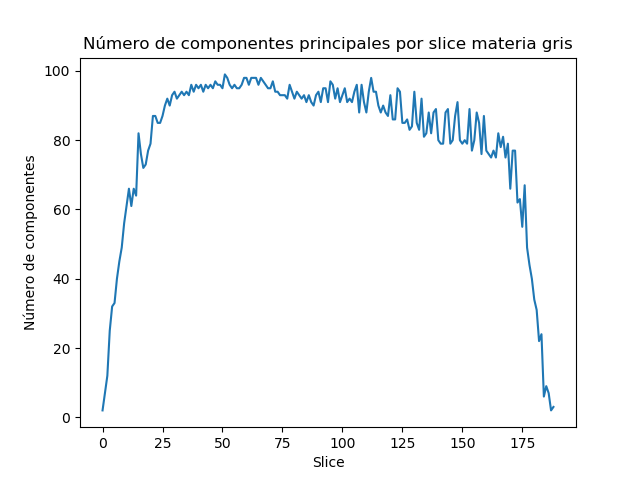
\includegraphics[scale=0.7]{pcc1.png}  %el parámetro scale permite agrandar o achicar la imagen. En el nombre de archivo puede especificar directorios
	\caption{Número de componentes principales por slice para C1} 
	\label{fig:pcc1}
\end{figure}

\begin{figure}[H] %con el [H] le obligamos a situar aquí la figura
	\centering
	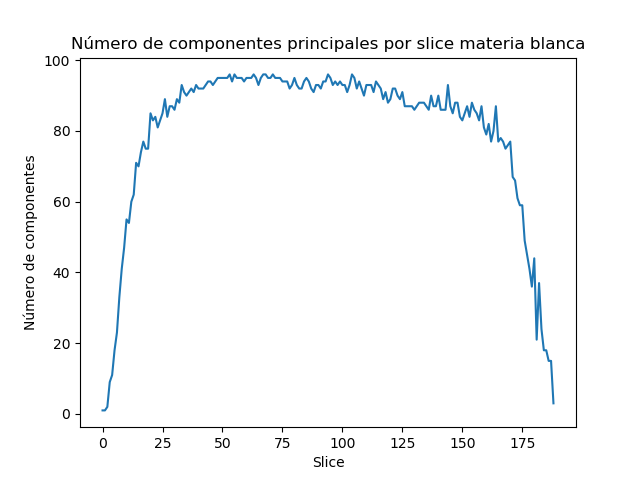
\includegraphics[scale=0.7]{pcc2.png}  %el parámetro scale permite agrandar o achicar la imagen. En el nombre de archivo puede especificar directorios
	\caption{Número de componentes principales por slice para C2} 
	\label{fig:pcc2}
\end{figure}

\subsubsection{Conclusiones}

La conclusión que extraemos es que ambos tipos de información tienen un comportamiento similar en rendimiento de clasificación. De entre el corte 0 a l 75 parece predominar la materia gris, y hasta el 189 la materia blanca obtiene ventaja. Se puede observar que la materia gris genera el máximo score entorno al corte 85. Además, desde el punto de vista estadístico, no se puede asegurar que una contenga más información relevante que la otra, por lo que optamos por seguir con toda la información del cerebro en los siguientes experimentos, a pesar de el incremento en el coste computacional que supone. 
\newpage
\subsection{Experimento 3}

En este experimento, utilizamos 242 (78 del grupo de control y 164 enfermos de PD) imágenes MRI para estudiar qué slices o cortes son las más determinantes a la hora de diagnosticar un paciente con Parkinson. A la luz del experimento 1, utilizamos plano Coronal como base y, por experimento 2, usamos la imagen completa del cerebro.

\subsubsection{Material y metodología}

Hacemos una partición de las imágenes. Por un lado, los pacientes que entran en juego en la primera fase de stacking (pacientes\_training) y, por otro, los que serán evaluados en la segunda fase (pacientes\_test). Todas las imágenes de los sujetos fueron, en primer lugar, segmentadas a través de la rutina de segmentación implementada en SPM12 (\cite{spm}). Tras ello, normalizamos y cambiamos el tamaño de la imagen a los bordes [-78 -112 -60; 78 76 85]. Extraemos características con la transformada discreta Wavelets 2D usando la transformada Bior3.3 hasta nivel 2. A continuación, realizo una normalización estándar de los coeficientes y, después, seleccionamos las características que explican el 95\% de la variabilidad en el conjunto de datos con PCA. Por último, el resultado de PCA fue ejecutado en SVM usando validación cruzada de 10 particiones y un conjunto de entrenamiento del 70\% de los datos. \\

Computamos los coeficientes wavelets 2D para cada slice, recopilamos toda la información en una matriz, generamos un modelos con SVM y el conjunto de training y, a continuación, hacemos una predicción con el conjunto de test, concluyendo la primera fase. Por tanto, hasta este momento, tenemos un nuevo dataset formado por las predicciones (valores 0 o 1) de un conjunto de pacientes de test, en el que en cada fila tenemos un paciente y cada columna corresponde a la predicción que nos ha dado cada slice sobre si el sujeto está enfermo o no (189 columnas). \\

En la segunda fase, dividimos de nuevo ese conjunto de datos final en entrenamiento y test (para evitar sobre aprendizaje) y, sobre la parte de train, aplico una regresión logística con validación cruzada de 10 particiones, para así poder valorar qué columnas (slices) tienen mayor peso a la hora del diagnóstico. Elijo un modelo lineal para poder conseguir una interpretabilidad mayor. Tras evaluar el modelo, conseguimos un accuracy total de 0.7 y, además, extraemos del mismo los pesos de cada slice para así poder ver cuáles son más determinantes.

\subsubsection{Resultados}

A parte del 0.7 en accuracy general, que no es un resultado que dé demasiada confianza, extraemos los 189 coeficientes asociados a los cortes y los parámetros del modelo. Nos centramos en los pesos. Son los siguientes:


\begin{figure}[H] %con el [H] le obligamos a situar aquí la figura
	\centering
	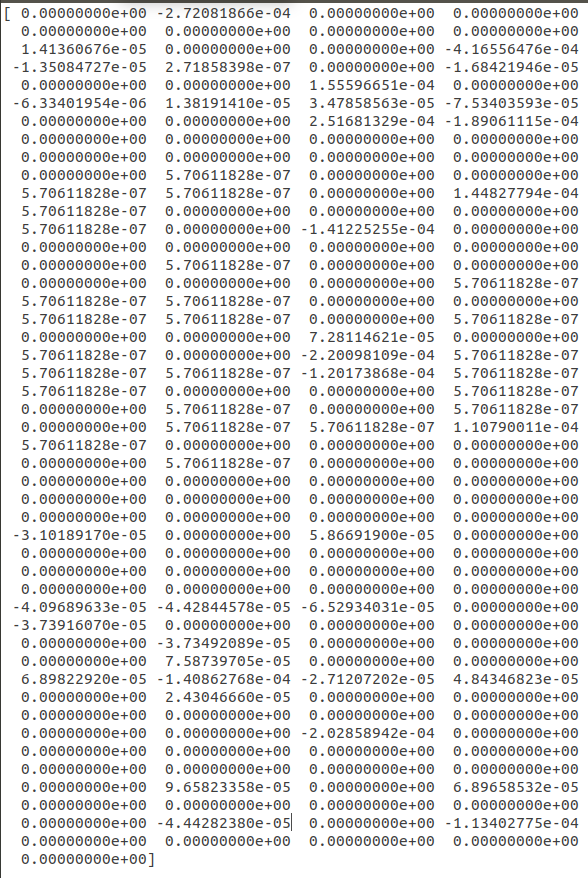
\includegraphics[scale=0.65]{probs-exp3.png}  %el parámetro scale permite agrandar o achicar la imagen. En el nombre de archivo puede especificar directorios
	\caption{Pesos asociados a cada slice en la regresión logística para el diagnóstico. Experimento 3} 
	\label{fig:probs-exp3}
\end{figure}

Como se puede observar, la mayoría de ellos son cero. Esto quiere decir que no aportan ninguna información en el diagnóstico (como cabría esperar, dado que, como se explicó en la sección 1, la enfermedad aparece en el mesencéfalo, en unas zonas muy concretas, por lo que un corte cercano a la parte superior de la cabeza no debería darnos información, por ejemplo), unos son positivos y otros negativos. Encontramos en la literatura el argumento de que aquellos coeficientes positivos más grandes son los que más información aportan para clasificar en la clase positiva, en nuestro caso, a los sujetos en el grupo de control. Por el contrario, aquellos coeficientes negativos que tienen mayor valor absoluto dan información al diagnóstico de enfermos. Por tanto, podemos darle una doble información al médico. En principio nos centramos en los coeficientes que dan información sobre el enfermo. Si tomamos los 10 mejores cortes, obtenemos:

$$[11, 1, 78, 162, 27, 50, 149, 82, 183, 23]$$

que se traduce, en una imagen cualquiera de un cerebro con plano Axial y Sagittal, en

\begin{figure}[H] %con el [H] le obligamos a situar aquí la figura
	\centering
	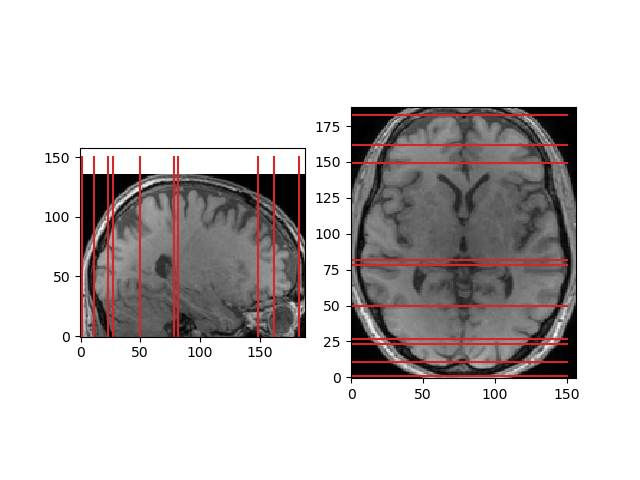
\includegraphics[scale=0.8]{cortes-PD-exp3.png}  %el parámetro scale permite agrandar o achicar la imagen. En el nombre de archivo puede especificar directorios
	\caption{Cortes más determinantes para Parkinson. Experimento 3} 
	\label{fig:cortes-PD-exp3}
\end{figure}

En el caso de los más determinantes para el grupo de control, encontramos 

$$[26, 18, 43, 95, 173, 145, 74, 148, 175, 118]$$

obteniendo la imagen

\begin{figure}[H] %con el [H] le obligamos a situar aquí la figura
	\centering
	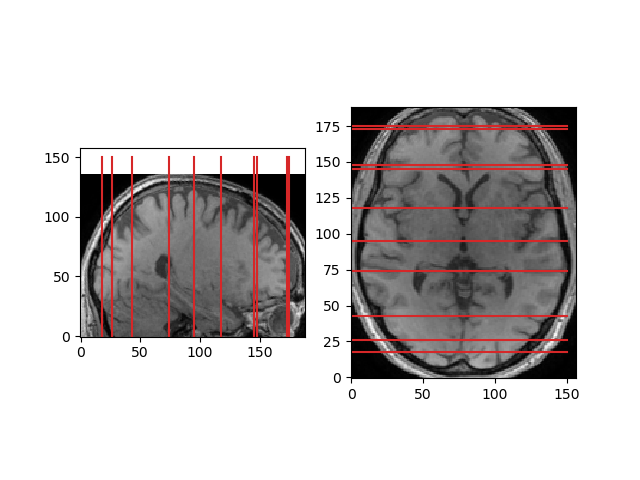
\includegraphics[scale=0.8]{cortes-C-exp3.png}  %el parámetro scale permite agrandar o achicar la imagen. En el nombre de archivo puede especificar directorios
	\caption{Cortes más determinantes para Control. Experimento 3} 
	\label{fig:cortes-C-exp3}
\end{figure}

Como no hay estudios médicos hasta la fecha sobre imágenes MRI y Parkinson, no podemos comprobar si los resultados se ajustan a certezas médicas. En \cite{alberto} se utilizan algoritmos genéticos en la optimización y se obtienen slices distintas. \\
\newpage
\textbf{Clasificación}

Hacemos una nueva clasificación incluyendo únicamente los slices vinculantes encontrados, utilizando el mismo preprocesamiento que antes y con un GridSearch de parámetros para SVM con validación cruzada de 10 particiones y 30\% de datos para el test (se puede encontrar en \textit{experimento3-bs.py}).Los resultados son los siguientes:

\begin{figure}[H] %con el [H] le obligamos a situar aquí la figura
	\centering
	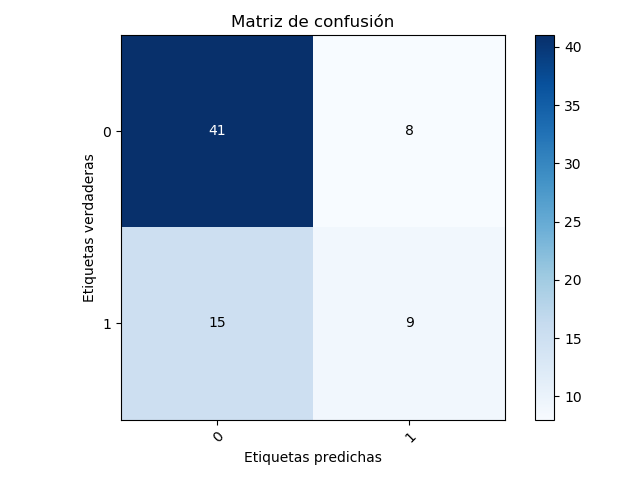
\includegraphics[scale=0.65]{conf2.png}  %el parámetro scale permite agrandar o achicar la imagen. En el nombre de archivo puede especificar directorios
	\caption{Matriz de confusión para la clasificación con los mejores cortes} 
	\label{fig:conf-mat-exp3}
\end{figure}

\begin{figure}[H] %con el [H] le obligamos a situar aquí la figura
	\centering
	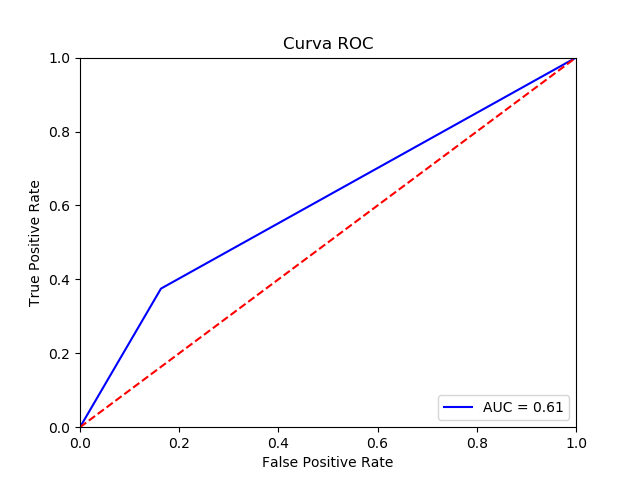
\includegraphics[scale=0.6]{roc2.png}  %el parámetro scale permite agrandar o achicar la imagen. En el nombre de archivo puede especificar directorios
	\caption{Curva ROC para la clasificación con los mejores cortes} 
	\label{fig:roc-exp3}
\end{figure}

Resultados para la predicción de Parkinson:

\begin{itemize}
	\item Precision: 0.73
	\item Recall: 0.84
	\item F1-Score: 0.78
\end{itemize}

 \newpage
\subsection{Experimento 4}

En este experimento, utilizamos 242 (78 del grupo de control y 164 enfermos de PD) imágenes MRI para estudiar qué slices o cortes son las más determinantes a la hora de diagnosticar un paciente con Parkinson. A la luz del experimento 1, utilizamos plano Coronal como base y, por experimento 2, usamos la imagen completa del cerebro.

\subsubsection{Material y metodología}

Volvemos a realizar la misma partición que en el experimento 3. Sin embargo, en esta ocasión no hacemos preprocesamiento alguno, buscando aprovechar las bondades de las redes neuronales profundas. La primera parte de los pacientes, para la fase uno del stacking, será utilizada para entrenar la red. Se genera un modelo por cada slice y se van almacenando las predicciones generadas con los elementos de la segunda fase. Dichas predicciones son evaluadas por la regresión logística con validación cruzada de 10 particiones para valorar los cortes más importantes según sus pesos, tal y como hicimos en el experimento anterior. \\

Antes de presentar los resultados, explico con detalle la topología de la red. Partimos de un modelo con dos capaz convolutivas que trabajan con la imagen completa (\cite{keras}):

\begin{figure}[H] %con el [H] le obligamos a situar aquí la figura
	\centering
	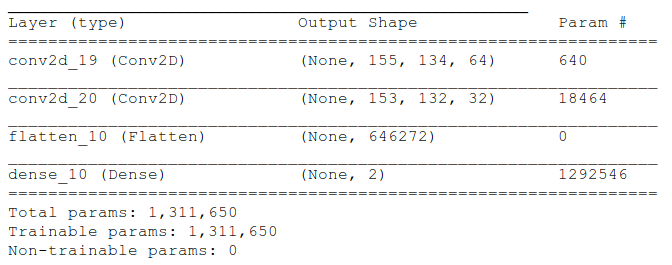
\includegraphics[scale=0.6]{conf1.png}  %el parámetro scale permite agrandar o achicar la imagen. En el nombre de archivo puede especificar directorios
	\caption{Configuración inicial de la red} 
	\label{fig:confnn1}
\end{figure}


Dado el número reducido de imágenes del que disponemos, parece excesivo tener más de 1.3 millones de parámetros ajustables por cada slice. A partir de aquí, añado capas de submuestreo (pooling) y una capa adicional densa. Además, reduzco el tamaño de la imagen con una tercera capa convolutiva (seguida de su capa de pooling):

\begin{figure}[H] %con el [H] le obligamos a situar aquí la figura
	\centering
	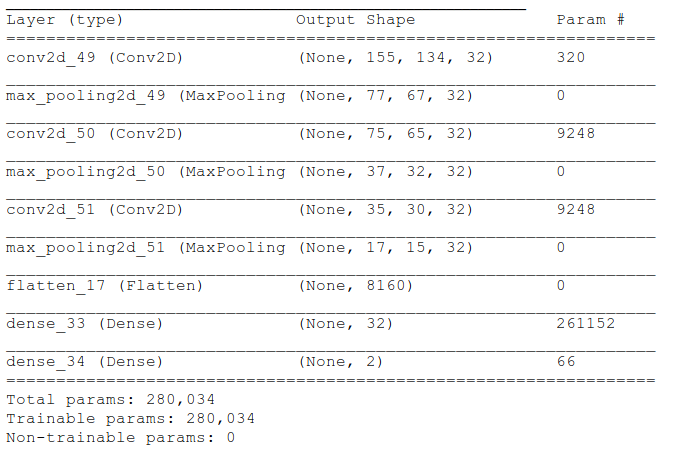
\includegraphics[scale=0.6]{confnn2.png}  %el parámetro scale permite agrandar o achicar la imagen. En el nombre de archivo puede especificar directorios
	\caption{Diseño de la red, parte 1} 
	\label{fig:confnn2}
\end{figure}



Aún así, siguen siendo demasiados parámetros para el tamaño del conjunto de datos que tenemos, por lo que reduzco aún más el tamaño de la red reduciendo su número de canales.

\begin{figure}[H] %con el [H] le obligamos a situar aquí la figura
	\centering
	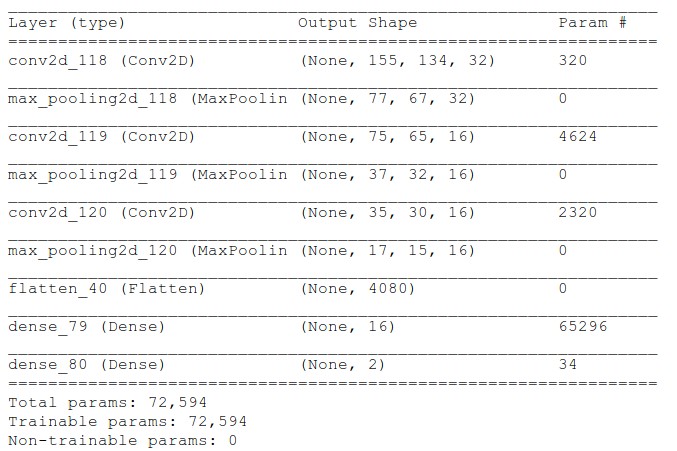
\includegraphics[scale=0.6]{confnn3.png}  %el parámetro scale permite agrandar o achicar la imagen. En el nombre de archivo puede especificar directorios
	\caption{Diseño de la red, parte 2} 
	\label{fig:confnn3}
\end{figure}


Fijo el número de épocas a 100. Por si la red no aprendiera lo suficiente en las primeras épocas, introduzco la posibilidad de detener el entrenamiento usando ``early stopping'', de forma que podemos ahorrar gran parte del tiempo de cálculo, ya que resultaría innecesario. 

\subsubsection{Resultados}

Obtenemos un 0.68 de accuracy en la validación cruzada. Estos son los coeficientes obtenidos para los 189 cortes:

\begin{figure}[H] %con el [H] le obligamos a situar aquí la figura
	\centering
	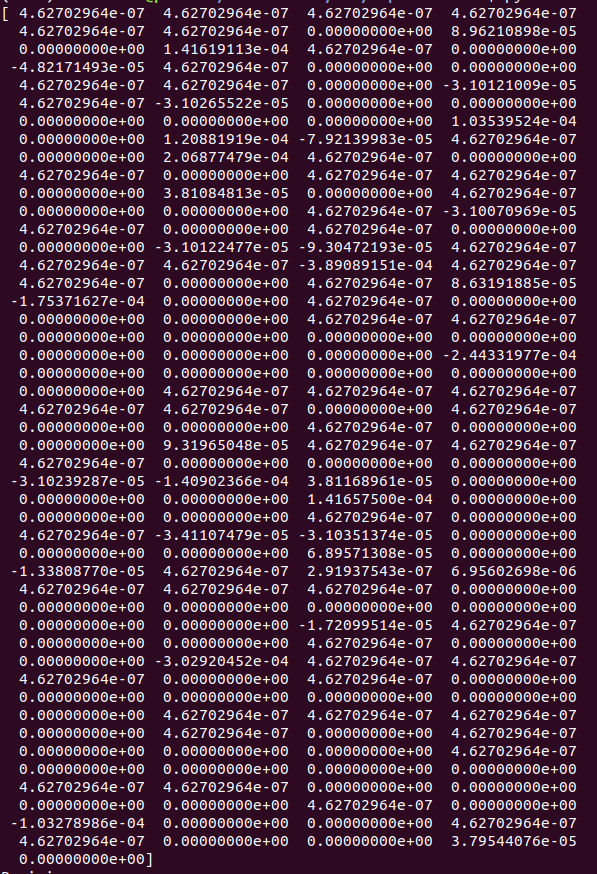
\includegraphics[scale=0.65]{probs-exp4.png}  %el parámetro scale permite agrandar o achicar la imagen. En el nombre de archivo puede especificar directorios
	\caption{Pesos asociados a cada slice en la regresión logística para el diagnóstico. Experimento 4} 
	\label{fig:probs-exp4}
\end{figure}

De nuevo, estudiamos los 10 mejores cortes para el diagnóstico del Parkinson y para el grupo de Control:

$$[58, 145, 79, 64, 105, 180, 54, 30, 12, 117]$$

\begin{figure}[H] %con el [H] le obligamos a situar aquí la figura
	\centering
	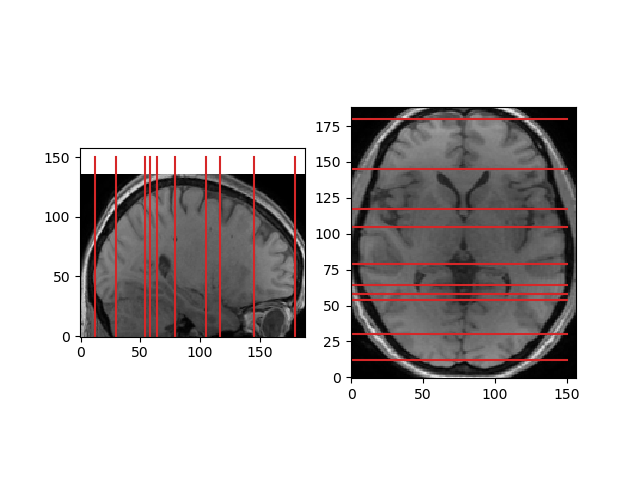
\includegraphics[scale=0.8]{cortes-PD-exp4.png}  %el parámetro scale permite agrandar o achicar la imagen. En el nombre de archivo puede especificar directorios
	\caption{Cortes más determinantes para Parkinson. Experimento 4} 
	\label{fig:cortes-PD-exp4}
\end{figure}

Para el grupo de Control,

$$[33, 110, 9, 29, 27, 97, 7, 63, 122, 106]$$

\begin{figure}[H] %con el [H] le obligamos a situar aquí la figura
	\centering
	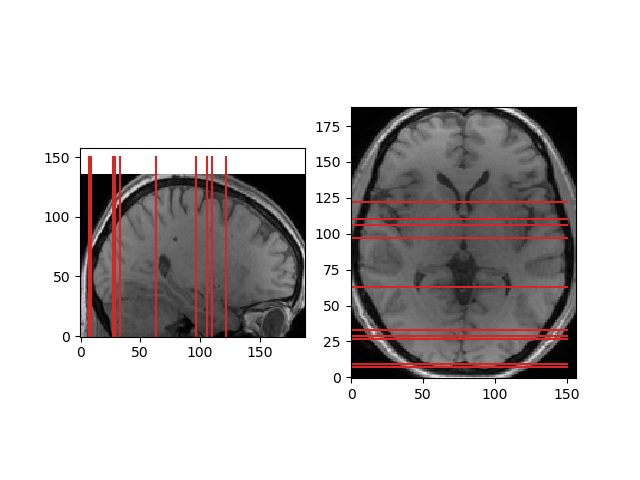
\includegraphics[scale=0.8]{cortes-C-exp4.png}  %el parámetro scale permite agrandar o achicar la imagen. En el nombre de archivo puede especificar directorios
	\caption{Cortes más determinantes para Control. Experimento 4} 
	\label{fig:cortes-C-exp4}
\end{figure}
\newpage
\textbf{CLASIFICACIÓN}

Realizamos una clasificación con el mismo propósito que en el experimento 3 (\textit{experimento4-bs.py}). Sin embargo, los resultados no han sido tan buenos. Basta ver la matriz de confusión para advertir que la red no ha conseguido aprender las características de la enfermedad con claridad:

\begin{figure}[H] %con el [H] le obligamos a situar aquí la figura
	\centering
	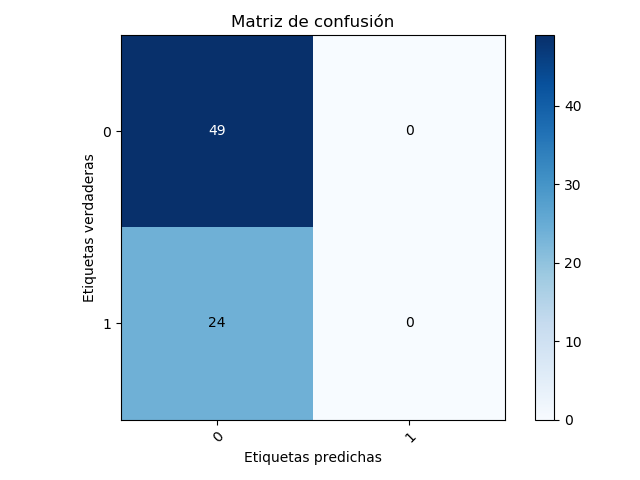
\includegraphics[scale=0.65]{conf-deeplearn1.png}  %el parámetro scale permite agrandar o achicar la imagen. En el nombre de archivo puede especificar directorios
	\caption{Matriz de confusión para la clasificación con los mejores cortes} 
	\label{fig:conf-mat-exp4}
\end{figure}

Como se puede ver, ha etiquetado a todos los elementos del test como si fueran enfermos, lo cuál es grave, ya que tendríamos gran cantidad de falsos positivos. A la luz de los resultados, no parece que deep learning pueda tener un buen rendimiento en un problema con tan pocos datos.

\newpage

\section{Desarrollo del proyecto software}

\subsection{Análisis y diseño}

\subsubsection{Subsistemas}

El sistema de información desarrollado se divide en 5 subsistemas, que son: Subsistema de normalización, Subsistema experimento 1, Subsistema experimento 2, Subsistema experimento 3 y Subsistema experimento 4. El primero de ellos es auxiliar y se encarga de normalizar, segmentar y generar las distintos tipos de fuentes de datos (C1, C2 y cerebro completo) para el resto de subsistemas. Los siguientes llevan a cabo cada uno de los experimentos descritos y justificados en la sección anterior. A continuación se presentan los requisitos de datos y funcionales del sistema completo.

\subsubsection{Requisitos de datos}

\begin{itemize}
	\item[R.D. 1:] Imágenes en bruto de MRI 3D en formato .nii (originalmente DICOM y transformado después).
	\item[R.D. 2:] Imágenes segmentadas y normalizadas en formato .nii con tres tipos de información: materia blanca, gris y cerebro completo.
	\item[R.D. 3:] Imágenes preprocesadas C1.
	\item[R.D. 4:] Imágenes preprocesadas C2.
	\item[R.D. 5:] Imágenes preprocesadas cerebro completo.
	\item[R.D. 6:] Características vía coeficientes de transformada discreta Wavelet 2D.
	\item[R.D. 7:] Características vía PCA.
	\item[R.D. 8:] Resultados de los experimentos: Gráficas, datos, valores de rendimiento, medidas.
	\item[R.D. 9:] Predicciones sobre el conjunto de test en stacking (2ª fase).
\end{itemize}

\subsubsection{Requisitos funcionales}

\begin{itemize}
	\item[R.F. 1:] Normalizar y segmentar las imágenes.
	\begin{itemize}
		\item Datos de entrada: R.D.1
		\item Datos de salida: R.D.2
	\end{itemize}
	\item[R.F. 2:] Extracción de características con wavelets 2D.
	\begin{itemize}
		\item Datos de entrada: R.D.2
		\item Datos de salida: R.D.6
	\end{itemize}
	\item[R.F. 3] Selección de características con PCA.
	\begin{itemize}
		\item Datos de entrada: R.D.6
		\item Datos de salida: R.D.7
	\end{itemize}
	\item[R.F. 4] Obtención del mejor plano.
	\begin{itemize}
		\item Datos de entrada: R.D.7
		\item Datos de salida: R.D.8
	\end{itemize}
	\item[R.F. 5] Obtención de la mejor fuente de información.
	\begin{itemize}
		\item Datos de entrada: R.D.7 (vía R.D. 3, 4 y 5)
		\item Datos de salida: R.D.8
	\end{itemize}
	\item[R.F. 6] Optimización de slices.
	\begin{itemize}
		\item Datos de entrada: R.D.9
		\item Datos de salida: R.D.8
	\end{itemize}
\end{itemize}

\subsubsection{Diagramas}
\vspace{1.5cm}
\textbf{ESQUEMA DE CAJA NEGRA}

\begin{figure}[H] %con el [H] le obligamos a situar aquí la figura
	\centering
	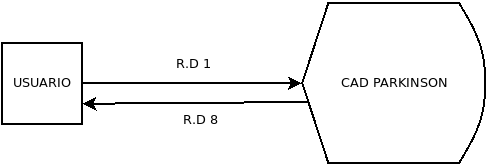
\includegraphics[scale=0.7]{esquema-cajanegra.png}  %el parámetro scale permite agrandar o achicar la imagen. En el nombre de archivo puede especificar directorios
	\caption{Esquema de caja negra} 
	\label{fig:caja-negra}
\end{figure}
\newpage
\textbf{ESQUEMA F-ARMAZÓN}

\begin{figure}[H] %con el [H] le obligamos a situar aquí la figura
	\centering
	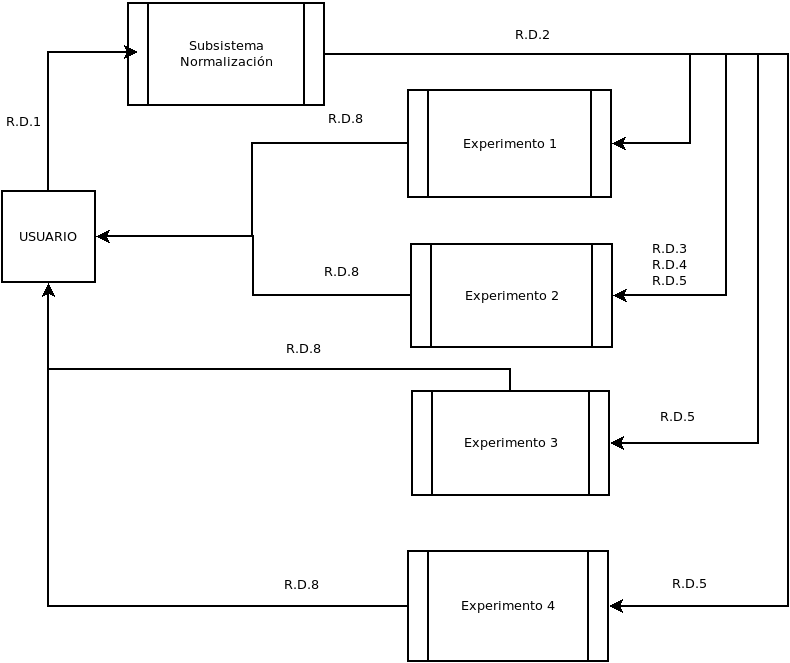
\includegraphics[scale=0.45]{esquema-f-armazon.png}  %el parámetro scale permite agrandar o achicar la imagen. En el nombre de archivo puede especificar directorios
	\caption{Esquema F-Armazón de los subsistemas} 
	\label{fig:f-armazon}
\end{figure}

\vspace{0.1cm}
\textbf{FLUJO DE DATOS EXPERIMENTO 1}

\vspace{0.5cm}
\begin{figure}[H] %con el [H] le obligamos a situar aquí la figura
	\centering
	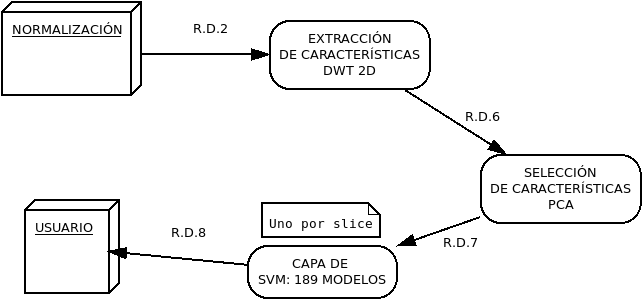
\includegraphics[scale=0.45]{fdexp1.png}  %el parámetro scale permite agrandar o achicar la imagen. En el nombre de archivo puede especificar directorios
	\caption{Esquema de flujo de datos para Experimento 1} 
	\label{fig:fdexp1}
\end{figure}

\newpage
\textbf{FLUJO DE DATOS EXPERIMENTO 2}
\vspace{0.5cm}

\begin{figure}[H] %con el [H] le obligamos a situar aquí la figura
	\centering
	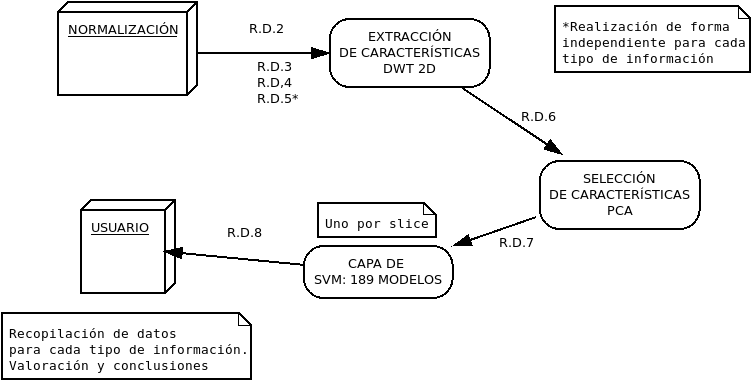
\includegraphics[scale=0.45]{fdexp2.png}  %el parámetro scale permite agrandar o achicar la imagen. En el nombre de archivo puede especificar directorios
	\caption{Esquema de flujo de datos para Experimento 2} 
	\label{fig:fdexp2}
\end{figure}

\vspace{1cm}
\textbf{FLUJO DE DATOS EXPERIMENTO 3}
\vspace{0.5cm}

\begin{figure}[H] %con el [H] le obligamos a situar aquí la figura
	\centering
	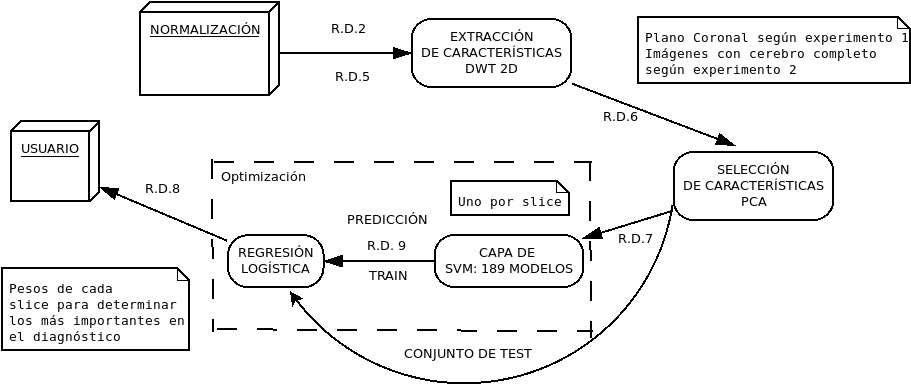
\includegraphics[scale=0.45]{fdexp3.png}  %el parámetro scale permite agrandar o achicar la imagen. En el nombre de archivo puede especificar directorios
	\caption{Esquema de flujo de datos para Experimento 3} 
	\label{fig:fdexp3}
\end{figure}
\newpage
\textbf{FLUJO DE DATOS EXPERIMENTO 4}
\vspace{0.5cm}

\begin{figure}[H] %con el [H] le obligamos a situar aquí la figura
	\centering
	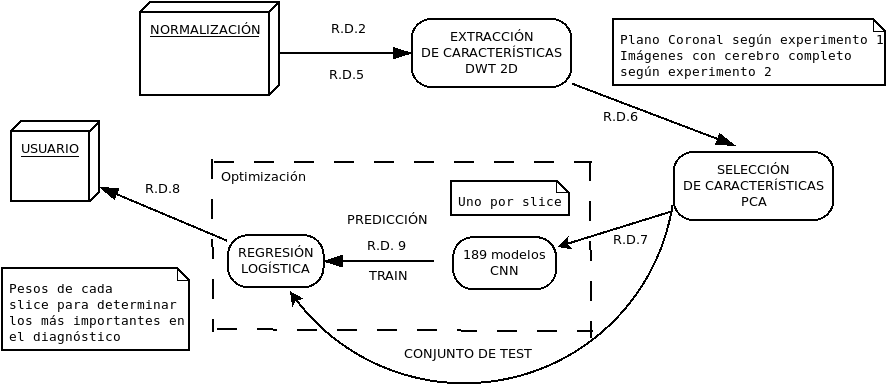
\includegraphics[scale=0.45]{fdexp4.png}  %el parámetro scale permite agrandar o achicar la imagen. En el nombre de archivo puede especificar directorios
	\caption{Esquema de flujo de datos para Experimento 4} 
	\label{fig:fdexp4}
\end{figure}

\subsection{Implementación}

Este proyecto software tiene licencia GNU General Public License v3.0, y todo su contenido se encuentra en mi repositorio \textit{https://github.com/luisbalru/TFG}. La totalidad de su desarrollo se ha hecho en Python a excepción del subsistema de normalización en el que empleo Matlab, ya que no encontré las herramientas necesarias ni las bibliotecas en Python. Como bibliotecas especiales, cabe destacar SPM12 (\cite{spm}) para la normalización y segmentación, Nibabel para lectura de neuroimágenes, SKlearn en general para todo el tratamiento, pywt para la extracción de características con DWT 2D, TensorFlow y Keras para la parte de Deep Learning. Para su utilización, basta con ejecutar los distintos ficheros ``experimento\_num-exp.py'' con la previa instalación de las dependencias. No necesita ningún argumento de entrada y se ejecuta sobre las imágenes situadas en las carpeta \textit{Datos/PD} o \textit{Datos/Control} para pacientes enfermos y sanos, respectivamente. Los resultados de los experimentos se guardan en ficheros de texto en el mismo directorio donde se encuentran los fuentes y son interpretados con los ``res-exp-num-exp.py'', apareciendo por pantalla las gráficos y/o resultados numéricos de precisión. 
\newpage

\section{Conclusiones y proyectos futuros} 

\subsection{Conclusiones}

El sistema de ayuda al diagnóstico del Parkison desarrollado ha constado de cuatro experimentos destinados al incremento paulatino de nuestro conocimiento sobre la enfermedad y el funcionamiento del cerebro. El primero de ellos estaba destinado a, de entre los tres cortes posibles que podemos hacer para obtener una imagen de dos dimensiones (axial, coronal y sagittal), cuál es más representativa. Nuestro resultado fue contundente: el plano coronal es el más informativo de todos ellos para esta demencia. El siguiente, que tenía propósito de ahorrar coste computacional, consistía en decidir si podíamos prescindir de una parte de la imagen completa del cerebro, quedándonos con la materia gris (C1) o la materia blanca (C2). Los resultados no fueron concluyentes, por lo que optamos por tomar siempre la imagen completa, a fin de garantizar la información más rica y los resultados más interesantes posibles. El tercer experimento tenía como objetivo primordial darle respuesta a la pregunta de qué corte, de los 189 que genera el plano coronal, contiene mayor información de interés en el diagnóstico de la enfermedad del Parkinson. Como es obvio, esta es nuestra pregunta central y el objeto de todo nuestro estudio. En la sección de experimentos se detallan los resultados, pero se puede decir que nuestro sistema es capaz de seleccionar las 10 slices más importantes y detecta a pacientes enfermos con una precisión del 73\% y un recall del 84\%. El experimento 4 estaba dedicado a la optimización vía deep learning de nuestro sistema. A pesar de que los resultados no han sido buenos, el diseño de la red ha sido enriquecedor y construye una nueva vía para el desarrollo de la biomedicina y el diagnóstico de enfermedades neurodegenerativas. 

\subsection{Proyectos futuros}

Existen trabajos pioneros (\cite{irojas}) que tratan de diagnosticar enfermedades neurodegenerativas trabajando con imágenes completas en 3D y no por cortes. La extensión de este trabajo de software libre a ese terreno sería un proyecto futuro muy interesante y viable, haciendo así herramientas abiertas para toda la comunidad. Además, deberíamos plantearnos utilizar otro tipo de imágenes, ya que expertos en imagen y radiología me advirtieron que MRI no era la mejor fuente de información para el diagnóstico de esta enfermedad. El traslado de estas técnicas a imágenes más potentes puede darnos un salto de calidad y verosimilitud que por fin consiga convencer a los médicos de la importancia de estas herramientas. Nunca fue nuestro propósito hacer de médicos ni acallar su criterio, si no darles una alternativa en casos de duda. \\

Desde un punto de vista más técnico, los resultados del experimento 4 confirman que deep learning no responde bien a problemas en los que el número de datos es reducido. Optamos por no utilizar \textit{data augmentation} para no falsear los resultados ni aumentar las estadísticas. Por otra parte, la generación de 189 modelos de deep learning podría mejorarse creando una única red más ambiciosa, en la que gran mayoría de las capas (sobre todo las primeras) fueran comunes para todas las slices, ya que no hay grandes diferencias al principio. Sólo se dividirían en detalles muy concretos, para que así la red consiguiera aprender con más esmero. 
\newpage

\section{Código}

\subsection{Normalización}

\lstinputlisting[firstline=1, lastline=67]{ppmi-normalize.m}

\subsection{Sujetos}


\lstinputlisting[firstline=1, lastline=41]{subjects.py}

\subsection{Experimento 1}

\lstinputlisting[firstline=1, lastline=208]{experimento1.py}

\subsubsection{Resultados experimento 1}

\lstinputlisting[firstline=1, lastline=83]{resultados-exp1.py}

\subsection{Experimento 2}

\lstinputlisting[firstline=1, lastline=114]{experimento2.py}

\subsubsection{Resultados experimento 2}

\lstinputlisting[firstline=1, lastline=59]{resultados-exp2.py}

\subsection{Experimento 3}

\lstinputlisting[firstline=1, lastline=161]{experimento3.py}

\subsubsection{Resultados experimento 3}

\lstinputlisting[firstline=1, lastline=59]{res-exp3.py}

\subsubsection{Clasificación con los mejores cortes. Experimento 3}

\lstinputlisting[firstline=1, lastline=161]{experimento3-bs.py}

\subsection{Experimento 4}

\lstinputlisting[firstline=1, lastline=181]{experimento4earlyStopping.py}

\subsubsection{Resultados experimento 4}

\lstinputlisting[firstline=1, lastline=44]{res-exp4.py}

\subsubsection{Clasificación con los mejores cortes. Experimento 4}

\lstinputlisting[firstline=1, lastline=182]{experimento4-bs.py}

\newpage
\section{Bibliografía}

%------------------------------------------------

\bibliography{bibliografia} %archivo citas.bib que contiene las entradas 
\bibliographystyle{unsrt} % hay varias formas de citar

\end{document}


%----------------------------------------------------------------------------------------
%	ANEXOS
%----------------------------------------------------------------------------------------

\appendix
\clearpage
\addappheadtotoc
\appendixpage



\end{document} 


